\documentclass{article}	

\usepackage[utf8]{inputenc}
\usepackage{amsmath}
\usepackage[german]{babel}
\usepackage{amssymb}
\usepackage{amsxtra}
\usepackage[dvips]{epsfig,psfrag}
\usepackage{listings}
\usepackage{url}
\usepackage[numbers]{natbib}
%\usepackage{jurabib}
\usepackage{hyperref}
\usepackage{breakurl}
\usepackage{verbatim}
\usepackage[lofdepth,lotdepth]{subfig} 
\usepackage{xspace} % Für dynamische Zwischenräume
\usepackage{eurosym} % Für das €-Symbol
\usepackage{float}

\bibliographystyle{plainnat}

\newcommand{\refchapter}[1]{Kapitel~\ref{#1}}
\newcommand{\refsec}[1]{Sektion~\ref{#1}}
\newcommand{\refeqn}[1]{Gleichung~(\ref{#1})}
\newcommand{\reffig}[1]{Abbildung~\ref{#1}}

\newcommand{\naglib}{{\it NAG C Library}\xspace}

\newenvironment{narrow}[2]{% Für extra breite Bilder
  \begin{list}{}{%
  \setlength{\topsep}{0pt}%
  \setlength{\leftmargin}{#1}%
  \setlength{\rightmargin}{#2}%
  \setlength{\listparindent}{\parindent}%
  \setlength{\itemindent}{\parindent}%
  \setlength{\parsep}{\parskip}}%
\item[]}{\end{list}}

\captionsetup[subfigure]{format=hang,margin=10pt,singlelinecheck=true}

\title{
{\bf \scriptsize RHEINISCH-WESTF\"ALISCHE TECHNISCHE HOCHSCHULE AACHEN \\
LuFG Informatik 12 (Prof. Dr. rer. nat. Uwe Naumann)}
\vspace{.5cm} \\

\epsfig{file=figures/STCE_Logo_WWW.eps,width=.7\textwidth}
\vspace{1cm} \\
{\bf \Large Korrelation und Regressionsanalyse} \\
{\large Seminararbeit} 
}

\author{vorgelegt von Patrick Neidig (Matr.-Nr. 272582)\\
	und Marius Grysla (Matr.-Nr. 274047)}

\begin{document}

\lstloadlanguages{[ISO]C++}
\lstset{basicstyle=\small, numbers=left, numberstyle=\footnotesize,
  stepnumber=1, numbersep=5pt, breaklines=true, escapeinside={/*@}{@*/}}


\pagestyle{headings}

\maketitle

\newpage
\tableofcontents

\newpage

\section{Einleitung}

Im Rahmen dieser Arbeit werden wir uns mit den Funktionen beschäftigen, welche die {\it NAG C Library}, eine Sammlung numerischer Algorithmen der {\it Numerical Algorithms Group} (kurz {\it NAG}) für die Programmiersprache {\it C}/{\it C++}, ihren Anwendern zur {\it Korrelation} und zur {\it Regressionsanalyse} zur Verfügung stellt.

Die Begriffe "`Korrelation"' und "`Regressionsanalyse"' stammen aus der {\it deskriptiven Statistik}, welche sich mit der Beschreibung, Darstellung und Analyse von Daten und Datensätzen befasst, die zuvor durch Erhebungen (z.B. Befragungen) oder Experimente gewonnen wurden.

Ein Beispiel für eine Erhebung wäre etwa die sog. {\it Studentische Lehrveranstaltungsbewertung}, die an der {\it RWTH Aachen} regelmäßig durchgeführt wird. Die bei Erhebungen oder Experimenten gewonnenen Daten umfassen {\it Merkmale} bestimmter {\it Merkmalsträger}: In unserem Beispiel wären die Merkmalsträger unter anderem die Studenten, die an der jeweiligen Erhebung teilnehmen, da sie zu mehreren persönlichen Merkmale befragt werden -- nämlich zu ihrem Geschlecht, ihrem Fachsemester und ihrer Nationalität. Weitere Merkmalsträger sind selbstverständlich die jeweilige Lehrveranstaltung, der Dozent und die Rahmenbedingungen, deren unterschiedliche Merkmale von den Studenten bewertet werden. Die einzelnen Merkmale können verschiedene {\it Merkmalsausprägungen} annehmen: Das Merkmal "`Fachsemester"' eines Studenten kann etwa die Ausprägungen "`1-2"', "`3-4"', "`5-6", "`7-8", "`9-10"' oder "`über 10"' annehmen. Die Merkmale der Lehrveranstaltung und des Dozenten können von den Studenten überwiegend auf einer fünfstufigen Skala von "`trifft völlig zu"' bis "`trifft nicht zu"' oder mit Noten von "`sehr gut"' bis "`mangelhaft"' bewertet werden, wodurch sie eben diese möglichen Ausprägungen haben. Die tatsächlichen Ausprägungen bzw. {\it Messwerte} aller Merkmale, die für einen einzelnen Merkmalsträger ermittelt wurden, werden in ihrer Gesamtheit {\it Beobachtung} genannt.

Anschließend an eine Erhebung oder ein Experiment lässt sich  der jeweils gewonnene Datensatz wie bereits erwähnt mit Hilfe der deskriptiven Statistik auf unterschiedliche Art und Weise beschreiben, darstellen und analysieren. Eine Möglichkeit ist es, ein einzelnes Merkmal zu betrachten und z.B. den Mittelwert der Noten zu berechnen, welche die Studenten der Lehrveranstaltung gegeben haben. Dies ist das Feld der {\it univariaten Statistik}. Eine weitere Möglichkeit ist es, zwei oder mehrere Merkmale gleichzeitig zu betrachten, um sie auf eventuelle Zusammenhänge zu prüfen. Es wäre etwa denkbar, dass das Merkmal "`Fachsemester"' eines Studenten und seine Bewertung des Merkmals "`Schwierigkeitsgrad"' der Lehrveranstaltung auf gewisse Weise zusammenhängen, was wichtig für die Interpretation der Messwerte des letzteren Merkmals wäre. Dies ist das Feld der {\it bi-} bzw. {\it multivariaten Statistik}. Hier sind schließlich auch die Korrelation und die Regressionsanalyse einzuordnen, welche sich beide mit der Beschreibung und Analyse zweier oder mehrerer Merkmale und ihres Zusammenhangs beschäftigen.

Zur Erläuterung der theoretischen Grundlagen der deskriptiven Statistik werden wir vorrangig auf Quelle \cite{Fahrmeir2010} zurückgreifen.

\subsection{Motivation}

Es ist natürlich nicht nur im Rahmen der {\it Studentischen Lehrveranstaltungsbewertung} an der {\it RWTH Aachen} interessant, die möglichen Zusammenhänge von Merkmalen festzustellen. Die Anwendungsbereiche der Korrelation und der Regressionanalyse erstrecken sich von der Wirtschaft (Wie wirken sich Werbemaßnahmen auf die Verkaufszahlen eines Produkts aus?) über die Medizin (Durch welche genetischen Veranlagungen wird eine Krankheit begünstigt?) bis hin zu Sozialwissenschaften (Wie wirken sich Bildungsmaßnahmen auf die Leistung von Schülern aus?) und natürlich auch Naturwissenschaften, um nur einige Beispiele zu nennen. Auf Grund der vielfachen Anwendung ist es wünschenswert und oft sogar nötig, solche statistischen Berechnungen automatisiert ausführen zu lassen, z.B. bei sehr großen Datensätzen. Die {\it NAG C Library} ist dabei ein wichtiges Hilfsmittel, stellt sie doch viele Funktionen für statistische Berechnungen bereits in fertiger Form zur Verfügung, so dass sie in beliebige Anwendungsprogramme integriert werden können -- vorausgesetzt, sie wurden in {\it C}/{\it C++} oder einer anderen unterstützten Programmiersprache geschrieben.

Zur Erklärung der implementierten Funktionen wird uns die Dokumentation der {\it NAG C Library} als haupsächliche Quelle dienen, insbesondere die Einleitung zum Kapitel {\it Correlation and Regression Analysis} \cite{nag:intro} sowie die Unterkapitel zu den jeweils vorgestellten Funktionen.

\subsection{Anwendungsbeispiel}

Weil statistische Beschreibungen und Analysen zwangsläufig Daten voraussetzen, die idealerweise repräsentativ sein sollten, werden wir in dieser Arbeit immer wieder auf den Datensatz {\it Münchner Mietspiegel 2003} zurückgreifen, welcher unter \cite{Fahrmeir2011} zu finden ist. Ein {\it Mietspiegel} dient Mietern, Vermietern und Mietberatungsstellen als Orientierungshilfe bei Mietfragen. Insbesondere lässt sich mit ihm die sog. {\it ortsübliche Vergleichsmiete}, d.h. die Nettomiete einer Wohnung in Abhängigkeit ihrer Größe, Art, Ausstattung, Beschaffenheit und Lage, ermitteln. Der vorliegende Mietspiegel ist ein Ausschnitt aus dem Mietspiegel der Stadt München im Jahr 2003, welchem eine repräsentative Zufallsstichprobe aus der Gesamtheit aller Wohnungen zu Grunde liegt.  Im Datensatz sind insgesamt 2053 Beobachtungen enthalten. Die interessierenden Merkmale wurden von Interviewern mit Hilfe von Fragebögen ermittelt. Welche dies im einzelnen sind, kann der Tabelle auf der folgenden Seite entnommen werden.

Zunächst jedoch noch ein kleiner Exkurs zum in der Tabelle erwähnten {\it Skalenniveau}, welches auch für die folgenden Kapitel von Bedeutung ist. Das Skalenniveau bezieht sich auf den Typ der Ausprägungen des jeweiligen Merkmals: Bilden die Ausprägungen eines Merkmals lediglich unabhängige Kategorien, wird es {\it nominalskaliert} genannt. Ein {\it dichotomes} Merkmal ist ein Sonderfall dieses Typs, der genau zwei Ausprägungen besitzt (im Beispiel immer "`ja"/"`nein"). Lassen sich die Ausprägungen außerdem nach einer logischen Reihenfolge ordnen, liegt ein {\it ordinalskaliertes} Merkmal vor. Können alle Ausprägungen zusätzlich als Zahlen interpretiert werden, deren Differenzen genau messar sind, so ist das Merkmal {\it intervallskaliert}. Besitzen die Ausprägungen schließlich auch noch einen natürlichen Nullpunkt, so dass sich ihr Verhältnis zueinander sinnvoll messen lässt, wird das Merkmal {\it verhältnisskaliert} genannt. Die letzten beiden Typen werden häufig auch als {\it metrisch} zusammengefasst.\\

\noindent {\bf Übersicht der Merkmale}\\

\noindent \begin{tabular}[ht]{|l|l|l|}
	\hline
	\textit{Name} & \textit{Beschreibung} & \textit{Skalenniveau}\\
	\hline \hline
	nm & Nettomiete in Euro & verhältnisskaliert\\ \hline
	nmqm & Nettomiete pro Quadratmeter in Euro & verhältnisskaliert\\ \hline
	wfl & Wohnfläche in Quadratmeter & verhältnisskaliert\\ \hline
	rooms & Anzahl der Zimmer & verhältnisskaliert\\ \hline
	bj & Baujahr & intervallskaliert\\ \hline
	bez & Stadtbezirk & nominalskaliert\\ \hline
	wohngut & gute Wohnlage & dichotom\\ \hline
	wohnbest & beste Wohnlage & dichotom\\ \hline
	ww0 & Warmwasserversorgung & dichotom\\ \hline
	zh0 & Zentralheizung & dichotom\\ \hline
	badkach0 & gekacheltes Bad & dichotom\\ \hline
	badextra & Zusatzausstattung im Bad & dichotom\\ \hline
	kueche & gehobene Küche & dichotom\\
	\hline
\end{tabular}\\\\

\noindent Der Übersichtlichkeit halber werden wir uns in dieser Arbeit auf den folgenden reduzierten Datensatz beziehen, welcher von uns zur Veranschaulichung konkreter Berechnungen zusammengestellt wurde:\\

\noindent {\bf Reduzierter Datensatz}\\

\noindent \begin{tabular}[ht]{|l|l|l|l|l|l|l|l|}
	\hline
	\textit{nm} & \textit{nmqm} & \textit{wfl} & \textit{rooms} & \textit{bj} & \textit{bez} & \textit{wohngut} & \textit{wohnbest}\\
	\hline \hline
	214,14 & 5,95 & 36 & 2 & 1948 & 17 & 0 & 0\\ \hline
	406,93 & 6,26 & 65 & 2 & 1966 & 10 & 0 & 0\\ \hline
	603,34 & 7,64 & 79 & 3 & 1986 & 13 & 1 & 0\\ \hline
	826,26 & 8,88 & 93 & 3 & 1918 & 5 & 1 &0\\ \hline
	1000,41 & 9,81 & 102 & 3 & 1918 & 8 & 0 & 0\\ \hline
	1227,12 & 10,14 & 121 & 5 & 1924 & 9 & 1 & 0\\ \hline
	1385,12 & 10,82 & 128 & 6 & 1991 & 9 & 1 & 0\\ \hline
	1661,55 & 11,08 & 150 & 5 & 1966 & 13 & 0 & 0\\
	\hline
\end{tabular}

\section{Korrelation}
\label{sec:korrelation}

Der Begriff {\it Korrelation} bezeichnet einen Zusammenhang zwischen zwei oder mehreren Merkmalen. Man sagt auch, dass diese Merkmale {\it korrelieren}. Wie stark dieser Zusammenhang ist, lässt sich messen, indem man verschiedene sog. {\it Korrelationskoeffizienten} berechnet \cite[S. 135]{Fahrmeir2010}. Im Folgenden werden wir zwei dieser Korrelationskoeffizienten mit Rückgriff auf Fahrmeir et al. \cite{Fahrmeir2010} vorstellen und im weiteren Verlauf der Arbeit näher untersuchen, wie ihre Berechnung in den entsprechenden Funktionen der {\it NAG C Library} implementiert ist und diese angewendet werden kann.

\subsection{Bravais-Pearson-Korrelationskoeffizient}
\label{sec:brav_pear_korr}

Der {\it Korrelationskoeffizient nach Bravais und Pearson} (auch {\it empirischer Korrelationskoeffizient} oder {\it Produkt-Moment-Korrelation} genannt) misst die Stärke des {\it linearen} Zusammenhangs zweier Merkmale $X$ und $Y$, die mindestens in intervallskalierter Form vorliegen müssen, und deren gegebenen Messwerten $x_1,x_2,...,x_n$ bzw. $y_1,y_2,...,y_n$ . Er ist wie folgt definiert \cite[S. 136]{Fahrmeir2010}:

\begin{equation*}
	r=\dfrac{s_{XY}}{s_Xs_Y}=\dfrac{\sum_{i=1}^{n}{(x_i-\bar{x})(y_i-\bar{y})}}{\sqrt{\sum_{i=1}^{n}{(x_i-\bar{x})^2\sum_{i=1}^{n}{(y_i-\bar{y})^2}}}} ~.
\end{equation*}

\noindent Dabei steht $\bar{x}$ bzw. $\bar{y}$ für die {\it arithmetischen Mittelwerte} der Merkmale $X$ und $Y$, $s_{X}$ bzw. $s_{Y}$ für ihre jeweiligen {\it Standardabweichungen} und $s_{XY}$ für ihre {\it Kovarianz}. Diese sind wiederum wie folgt definiert \cite[S. 136]{Fahrmeir2010}:\\

\noindent {\bf Arithmetischer Mittelwert}
\begin{equation*}
	\bar{x}=\dfrac{1}{n}\sum_{i=1}^{n}{x_i}=\dfrac{1}{n}(x_1+...+x_n) ~.
\end{equation*}

\noindent {\bf Standardabweichung}
\begin{equation*}
	s_X=\sqrt{\dfrac{1}{n}\sum_{i=1}^{n}{(x_i-\bar{x})^2}}=\sqrt{\dfrac{1}{n}(x_1-\bar{x})^2+...+(x_n-\bar{x})^2} ~.
\end{equation*}

\noindent {\bf Kovarianz}
\begin{equation*}
	s_{XY}=\dfrac{1}{n}\sum_{i=1}^{n}{(x_i-\bar{x})(y_i-\bar{y})}=\dfrac{1}{n}(x_1-\bar{x})(y_1-\bar{y})+...+(x_n-\bar{x})(y_n-\bar{y}) ~.
\end{equation*}

\noindent Dabei lassen sich $\bar{y}$ und $s_{Y}$ analog zu $\bar{x}$ und $s_{X}$ berechnen. Der gültige Wertebereich von $r$ ist $-1 \leq r \leq +1$ und folgendermaßen zu interpretieren \cite[S. 137]{Fahrmeir2010}:
\begin{itemize}
    \item $r>0$: Positive Korrelation: Es besteht ein gleichsinniger linearer Zusammenhang zwischen den Merkmalen, d.h. alle Paare $(x_i, y_i)$ mit $i=1,...,n$ der Merkmalsausprägungen bilden annähernd eine Gerade mit positiver Steigung.
    \item $r<0$: Negative Korrelation: Es besteht ein gegensinniger linearer Zusammenhang zwischen den Merkmalen, d.h. alle Paare bilden annähernd eine Gerade mit negativer Steigung.
    \item $r=0$: Keine Korrelation: Es besteht kein linearer Zusammenhang.
\end{itemize}

\noindent Für positive und negative Korrelation ist zu beachten, dass sie üblicherweise in verschiedene Stärkeklassen eingeteilt werden \cite[S. 139]{Fahrmeir2010}: Gilt $0<|r|<0,5$, so spricht man von einer schwachen Korrelation, d.h. der Zusammenhang zwischen den Merkmale ist sehr gering. Hier ist in Frage zu stellen, ob es sich überhaupt um eine Korrelation handelt. Eine mittlere Korrelation liegt erst für $0,5 \leq |r| < 0,8$ und eine starke für $0,8 \leq |r| \leq 1$ vor, d.h. es kann von einem signifikanten Zusammenhang zwischen den Merkmalen und somit von einer Korrelation ausgegangen werden. Dies liefert allerdings noch keinen Hinweis darauf, ob die Merkmale auch kausal zusammenhängen. Hierzu liefert die partielle Korrelation genauere Informationen (siehe Sektion \ref{sec:part_korr}).

Liegen die Merkmale, deren Korrelation ermittelt werden soll, nicht in intervallskalierter, sondern nur in ordinalskalierter Form vor, kann auf den Spearman-Korrelationskoeffizienten zurückgegriffen werden (siehe \refsec{sec:spear_rangkorr}).

\subsubsection{NAG-Funktion}
\label{sec:brav_pear_korr_funk}

In der {\it NAG C Library} kann der Bravais-Pearson-Korrelationskoeffizient zweier mindestens intervallskalierter Merkmale mit Hilfe der Funktion {\it nag\_corr\_cov()} berechnet werden, welche wir nun unter Berücksichtigung der Dokumentation \cite{nag:g02bxc} näher betrachten werden. Sie ist folgendermaßen spezifiziert \cite[S. 1]{nag:g02bxc}:\\

\noindent void nag\_corr\_cov (Integer $n$, Integer $m$, const double $x[]$, Integer $tdx$,\\
\hspace*{5mm} const Integer $sx[]$, const double $wt[]$, double *$sw$, double $wmean[]$,\\
\hspace*{5mm} double $std[]$, double $r[]$, Integer $tdr$, double $v[]$, Integer $tdv$,\\
\hspace*{5mm} NagError *$fail$)\\

\noindent Die Parameter der Funktion sind in Eingabe- und Ausgabe-Parameter unterteilt und werden in den folgenden beiden Tabellen erklärt \cite[S. 2-3]{nag:g02bxc}:\\

\noindent {\bf Eingabe-Parameter}\\

\noindent \begin{tabular}[ht]{|l|l|}
  	\hline
  	\textit{Name} & \textit{Beschreibung}\\
  	\hline \hline
  	$n$ & Anzahl der Beobachtungen im Datensatz ($n > 1$)\\ \hline
  	$m$ & Anzahl der Merkmale im Datensatz ($m \geq 1$)\\ \hline
	$x[n \times tdx]$ & Datenmatrix: $x[i - 1][j - 1]$ enthält die $i$-te Beobachtung\\
	& des $j$-ten Merkmals\\ \hline
	$tdx$ & Zeilenlänge der Datenmatrix $x$ ($tdx \geq m$)\\ \hline
	$sx[m]$ & gibt für jedes Merkmal an, ob es in die Analyse einbezogen\\
	& wird ($sx[j-1] \geq 0$): einbezogen falls $sx[j-1] > 0$, sonst nicht\\ \hline
	$wt[n]$ & gibt für jede Beobachtung ein Gewicht an ($wt[i-1] \geq 0$)\\ \hline
	$tdr$, $tdv$ & beide analog zu $tdx$\\
	\hline
\end{tabular}\\\\

\newpage

\noindent {\bf Ausgabe-Parameter}\\
	
\noindent \begin{tabular}[ht]{|l|l|}
  	\hline
  	\textit{Name} & \textit{Beschreibung}\\
  	\hline \hline
	$sw$ & Summe der Gewichte falls $wt$ gesetzt, sonst gleich $n$\\ \hline
  	$wmean[m]$ & Arithmetische Mittelwerte: $wmean[j - 1]$ enthält\\
  	& den arithmetischen Mittelwert für das $j$-te Merkmal\\ \hline
  	$std[m]$ & Standardabweichungen: $std[j - 1]$ enthält die\\
  	& Standardabweichung für das $j$-te Merkmal\\ \hline
  	$r[m \times tdr]$ & Korrelationsmatrix: $r[j - 1][k - 1]$ enthält den\\
	& Korrelationskoeffizienten nach Bravais und Pearson\\
	& für die Merkmale $j$ und $k$\\ \hline
	$v[m \times tdv]$ & Kovarianzmatrix: $v[j - 1][k - 1]$ enthält die\\
	& Kovarianz zwischen den Merkmalen $j$ und $k$\\
  	\hline
\end{tabular}\\\\

\noindent {\bf Algorithmus}\\

\noindent Der Algorithmus der Funktion berechnet aus der übergebenen Datenmatrix $x$ sukzessive die arithmetischen Mittelwerte (separat), Standardabweichungen (separat) sowie die Kovarianzen (paarweise) für alle Merkmale, die über $sx$ einbezogen wurden, und gibt sie über die jeweiligen Parameter aus. Dabei werden ggf. in $wt$ angegebene Gewichte für die Messwerte der Beobachtungen berücksichtigt (was hier auf Grund der Beschränkung der Arbeit vernachlässigt wird). An den Formeln in \refsec{sec:brav_pear_korr} lässt sich bereits erkennen, dass eine sukzessive Vorgehensweise nötig ist, da die einzelnen Berechnungen die jeweils vorherige Berechnung voraussetzen und somit aufeinander aufbauen. Abschließend wird für alle einbezogenen Merkmale paarweise der Bravais-Pearson-Korrelationskoeffizient berechnet und als Korrelationsmatrix $r$ ausgegeben \cite[S. 1]{nag:g02bxc}.

In der nächsten Sektion wird dies an unserem Beispiel nochmals verdeutlicht.

\subsubsection{Anwendung}
\label{sec:brav_pear_korr_anw}

Angenommen, wir wollen feststellen, welche intervall- und verhältnisskalierten Merkmale des Beispieldatensatzes mindestens mittel ($|r|>0,5$) oder sogar stark ($|r|>0,8$) korrelieren. Dazu übergeben wir der Funktion {\it nag\_corr\_cov()} als Eingabe für $x$ den reduzierten Datensatz und beziehen alle in Frage kommenden Merkmale (nämlich die ersten fünf, vgl. Tabelle in \refsec{sec:beispiel}) über $sx$ ein. Nun berechnet der Algorithmus im ersten Schritt zuerst für jedes Merkmal $X$ separat den arithmetischen Mittelwert, z.B. für die Nettomiete:
\begin{equation*}
	\bar{x}=\dfrac{1}{8}(214,14+406,93+603,34+826,26+...+1661,55)=915,61 ~.
\end{equation*}

\noindent Im zweiten Schritt wird ebenfalls für jedes Merkmal $X$ separat die Standardabweichung $s_X$ berechnet:
\begin{equation*}
	s_X=\sqrt{\dfrac{1}{8}(214,14-915,61)^2+...+(1661,55-915,61)^2}=466,02 ~.
\end{equation*}

\noindent Im dritten Schritt werden für alle Merkmale $X$ und $Y$ paarweise die Kovarianzen $s_{XY}$ berechnet, in der Kovarianzmatrix $v$ zusammengefasst und ausgegeben. Für Nettomiete und Wohnfläche ergibt sich z.B. folgende Rechnung:
\begin{equation*}
	\begin{split}
		s_{XY}=& \dfrac{1}{8}(214,14-915,61)(36-96,75)+...\\
		& +(1661,55-915,61)(150-96,75)=18147,94 ~.
	\end{split}
\end{equation*}

\noindent Im letzten Schritt berechnet der Algorithmus schließlich für alle Merkmale paarweise den Bravais-Pearson-Korrelationskoeffizienten und gibt die zusammengefassten Ergebnisse in der Korrelationsmatrix $r$ aus (hier nun für den gesamten Datensatz, d.h. alle Beobachtungen):
\begin{equation*}
	r =
	\begin{pmatrix}
		1,00 & 0,47 & {\bf 0,71} & {\bf 0,54} & 0,05\\
 		0,47 & 1,00 & -0,23 & -0,27 & 0,29\\
 		0,71 & -0,23 & 1,00 & {\bf 0,84} & -0,20\\
		0,54 & -0,27 & 0,84 & 1,00 & -0,15\\
  		0,05 &  0,29 & -0,20 & -0,15 & 1,00\\
	\end{pmatrix} ~.
\end{equation*}

\noindent An der Korrelationsmatrix lässt sich schließlich ablesen, welche Merkmale mittel bis stark korrelieren: Sowohl die $i$-te Zeile als auch die $i$-te Spalte der Matrix  entsprechen den Korrelationskoeffizienten für das $i$-te Merkmal, gepaart mit allen anderen Merkmalen und sich selbst. Die Matrix ist folglich symmetrisch, weshalb nur die obere Hälfte betrachtet werden muss, und enthält auf der Diagonalen "`perfekte" Korrelationen, da jedes Merkmal natürlich maximal mit sich selbst korreliert. Im Beispiel wurden die mittel bis stark korrelierenden Merkmale markiert: Sowohl Nettomiete und Wohnfläche als auch Wohnfläche und Anzahl der Räume korrelieren stark. Außerdem liegt eine mittlere Korrelation zwischen Nettomiete und Anzahl Räume vor.

\subsection{Spearman-Rangkorrelationskoeffizient}
\label{sec:spear_rangkorr}

Der {\it Rangkorrelationskoeffizient nach Spearman} misst die Stärke des {\it monotonen} Zusammenhangs zweier Merkmale $X$ und $Y$, die in mindestens ordinalskalierter Form vorliegen müssen, indem die ursprünglichen Messwerte vor der eigentlichen Berechnung in {\it Ränge} transformiert werden \cite[S. 142]{Fahrmeir2010}.

Dabei wird jedem $x_i$ für $i=1,...,n$ als Rang die Zahl der Position zugewiesen, die $x_i$ erhält, wenn man $x_1, x_2, ..., x_n$ der Größe nach ordnet. Für die so geordneten Messwerte $x_{(1)}<x_{(2)}<...<x_{(n)}$ gilt dann $rg(x_{(i)})=i$. Mit jedem $y_i$ für $i=1,...,n$ wird analog verfahren. Aus den ursprünglichen Messwertpaaren $(x_i, y_i)$ ergeben sich somit die neuen Rangpaare $(rg(x_i), rg(y_i))$ für $i=1,...,n$.

Treten Messwerte doppelt auf, ist die Rangvergabe nicht eindeutig. In einem solchen Fall werden deshalb sog. {\it Durchschnittsränge} gebildet, d.h. jedem der betroffenen Messwerte wird als Rang der arithmetische Mittelwert der potentiellen Ränge zugewiesen. Ein Beispiel: In einem Datensatz liegen drei gleiche Merkmalsausprägungen vor, welche die Ränge 5, 6 und 7 belegen könnten. Weil sie jedoch nicht eindeutig der Größe nach angeordnet werden können, erhalten alle drei den Durchschnittsrang $rg=(5+6+7):3=6$.

Der eigentliche Rangkorrelationseffizient wird schließlich ermittelt, indem der Korrelationskoeffizient nach Bravais und Pearson für die transformierten Rangpaare $(rg(x_i), rg(y_i))$ für $i=1,...,n$ berechnet wird. Er ist somit wie folgt definiert:

\begin{equation*}
    r_{SP}=\dfrac{\sum_{i=1}^{n}{(rg(x_i)-\bar{rg}_X)(rg(y_i)-\bar{rg}_Y)}}{\sqrt{\sum_{i=1}^{n}{(rg(x_i)-\bar{rg}_X)^2\sum_{i=1}^{n}{(rg(y_i)-\bar{rg}_Y)^2}}}} \quad ,
\end{equation*}

\noindent wobei $\bar{rg}_X$ und $\bar{rg}_Y$ für die arithmetischen Mittelwerte aller Ränge der Merkmale $X$ und $Y$ stehen \cite[S. 142-143]{Fahrmeir2010}. Der gültige Wertebereich von $r_{SP}$ ist gleich dem Wertebereich von $r$ und analog zu interpretieren \cite[S. 143]{Fahrmeir2010}.

\subsubsection{NAG-Funktion}
\label{sec:spear_rangkorr_funk}

In der {\it NAG C Library} kann der Spearman-Korrelationskoeffizient zweier mindestens ordinalskalierter Merkmale mit Hilfe der Funktion {\it nag\_ken\_spe\_corr\_coeff()} berechnet werden \cite{nag:g02brc}. Wie ihr Name schon andeutet, wird mit dieser Funktion ebenfalls der {\it Kendall-Rangkorrelationskoeffizient} berechnet, welcher allerdings auf Grund der Beschränkung dieser Arbeit vernachlässigt wird. Sie ist wie folgt spezifiziert \cite[S. 1]{nag:g02brc}:\\

\noindent void nag\_ken\_spe\_corr\_coeff (Integer $n$, Integer $m$, const double $x[]$, Integer $tdx$,\\
\hspace*{5mm} const Integer $svar[]$, const Integer $sobs[]$, double $corr[]$, Integer $tdc$,\\
\hspace*{5mm} NagError *$fail$)\\

\noindent Die Parameter der Funktion sind ebenfalls in Eingabe- und Ausgabe-Parameter unterteilt, die in in den folgenden Tabellen erläutert werden \cite[S. 2-3]{nag:g02brc}:\\

\noindent {\bf Eingabe-Parameter}\\

\noindent \begin{tabular}[ht]{|l|l|}
  	\hline
  	\textit{Name} & \textit{Beschreibung}\\
  	\hline \hline
  	$n$ & Anzahl der Beobachtungen im Datensatz ($n > 1$)\\ \hline
  	$m$ & Anzahl der Merkmale im Datensatz ($m \geq 2$)\\ \hline
	$x[n \times tdx]$ & Datenmatrix: $x[i - 1][j - 1]$ enthält die $i$-te\\
	& Beobachtung des $j$-ten Merkmals\\ \hline
	$tdx$ & Zeilenlänge der Datenmatrix $x$ ($tdx \geq m$)\\ \hline
	$svar[m]$ & gibt für jedes Merkmal an, ob es in die Analyse\\
	& einbezogen wird: einbezogen falls $svar[j-1] > 0$,\\
	& sonst nicht ($svar[j-1] \geq 0$)\\ \hline
	$sobs[n]$ & gibt für jede Beobachtung an, ob sie in die Analyse\\
	& einbezogen wird:  einbezogen falls $sobs[i-1] > 0$, \\
	& sonst nicht ($sobs[i-1] \geq 0$)\\ \hline
	$tdc$ & analog zu $tdx$\\
	\hline
\end{tabular}\\\\

\newpage

\noindent {\bf Ausgabe-Parameter}\\
	
\noindent \begin{tabular}[ht]{|l|l|}
  	\hline
  	\textit{Name} & \textit{Beschreibung}\\
  	\hline \hline
  	$corr[m \times tdc]$ & Korrelationsmatrix: $r[j - 1][k - 1]$ enthält den\\
	& Korrelationskoeffizienten nach Spearman für die\\
	& Merkmale $j$ und $k$\\
  	\hline
\end{tabular}\\\\

\noindent {\bf Algorithmus}\\

\noindent Der Algorithmus der Funktion berechnet für die einbezogenen Messwerte der übergebenen Datenmatrix $x$ die entsprechenden Ränge und ermittelt auf Grundlage der neuen, transformierten Datenmatrix $x'$ analog zur oben bereits erläuterten Funktion {\it nag\_corr\_cov()} für alle einbezogenen Merkmale paarweise den Spearman-Rangkorrelationskoeffizienten. Abschließend werden die Ergebnisse zusammengefasst als Korrelationsmatrix $corr$ ausgegeben \cite[S. 1]{nag:g02brc}.

Dies wird in der nächsten Sektion wieder an unserem Beispiel verdeutlicht.

\subsubsection{Anwendung}
\label{sec:spear_rangkorr_anw}

Leider sind im Beispieldatensatz keine ordinalskalierten Merkmale vorhanden, so dass wir wieder feststellen werden, welche intervall- und verhältnisskalierten Merkmale korrelieren. Darüber hinaus können wir anschließend die ermittelten Spearman-Rangkorrelationskoeffizienten mit den bereits für die gleichen Merkmale berechneten Bravais-Pearson-Korellationskoeffizienten vergleichen. Dazu übergeben wir der Funktion {\it nag\_ken\_spe\_corr\_coeff()} als Eingabe für $x$ den reduzierten Datensatz und beziehen alle in Frage kommenden Merkmale (wieder die ersten fünf) über $svar$ ein. Nun berechnet der Algorithmus im zuerst für jeden Messwert $x_i$ jedes Merkmals $X$ den entsprechenden Rang $rg(x_i)$, z.B. für das Baujahr:
\begin{equation*}
	\begin{split}
		& x_{(1)}=1918 \Rightarrow rg(1918)=(1+2):2=1,5\\
		& x_{(2)}=1918 \Rightarrow rg(1918)=(1+2):2=1,5\\
		& x_{(3)}=1924 \Rightarrow rg(1924)=3\\
		& x_{(4)}=1948 \Rightarrow rg(1948)=4\\
		& x_{(5)}=1966 \Rightarrow rg(1966)=(5+6):2=5,5\\
		& x_{(6)}=1966 \Rightarrow rg(1966)=(5+6):2=5,5\\
		& x_{(7)}=1986 \Rightarrow rg(1986)=7\\
		& x_{(8)}=1991 \Rightarrow rg(1991)=8 ~.
	\end{split}
\end{equation*}

\noindent Für die gesamte Datenmatrix ergibt sich:
\begin{equation*}
	x =
	\begin{pmatrix}
		214,14 & 5,95 & 36 & 2 & 1948\\
		406,93 & 6,26 & 65 & 2 & 1966\\
		603,34 & 7,64 & 79 & 3 & 1986\\
		826,26 & 8,88 & 93 & 3 & 1918\\
		1000,41 & 9,81 & 102 & 3 & 1918\\
		1227,12 & 10,14 & 121 & 5 & 1924\\
		1385,12 & 10,82 & 128 & 6 & 1991\\
		1661,55 & 11,08 & 150 & 5 & 1966\\
	\end{pmatrix}
	\Rightarrow
	x' =
	\begin{pmatrix}
		1 & 1 & 1 & 1,5 & 4\\
		2 & 2 & 2 & 1,5 & 5,5\\
		3 & 3 & 3 & 4 & 7\\
		4 & 4 & 4 & 4 & 1,5\\
		5 & 5 & 5 & 4 & 1,5\\
		6 & 6 & 6 & 6,5 & 3\\
		7 & 7 & 7 & 8 & 8\\
		8 & 8 & 8 & 6,5 & 5,5\\
	\end{pmatrix} ~.
\end{equation*}

\noindent Danach wird aus der neuen Datenmatrix $x'$ analog zur Funktion {\it nag\_corr\_cov()} die Korrelationsmatrix $r$ berechnet. Diese wird schließlich als Korrelationsmatrix $corr$ mit den Spearman-Rangkorrelationskoeffizienten für alle Merkmalspaare ausgegeben (hier nun für den gesamten Datensatz, d.h. alle Beobachtungen):
\begin{equation*}
	corr =
	\begin{pmatrix}
		1 & 0,46 & {\bf 0,70} & {\bf 0,55} & 0,13\\
		0,33 & 1 & -0,23 & -0,28 & 0,30\\
		0,52 & -0,16 & 1 & {\bf 0,86} & -0,11\\
		0,43 & -0,21 & 0,74 & 1 & -0,12\\
		0,10 & 0,21 & -0,08 & -0,09 & 1\\
	\end{pmatrix} ~.
\end{equation*}

\noindent Hierbei ist zu beachten, dass die Spearman-Rangkorrelationskoeffizienten nur in oberen Hälfte abgelesen werden können. In der unteren Hälfte sind die automatisch gleichzeitig ermittelten Kendall-Rangkorrelationskoeffizienten zu sehen \cite[S. 2-3]{nag:g02brc}. Wie offensichlich zu erkennen ist, liegen die berechneten Rangkorrelationskoeffizienten nach Spearman insgesamt recht nah an den Korrelationskoeffizienten nach Bravais und Pearson (vgl. Matrix $r$ in Sektion \refsec{sec:brav_pear_korr_anw}).

\subsection{Partielle Korrellation}
\label{sec:part_korr}

An dieser Stelle sei noch erwähnt, dass eine vorhandene Korrelation zwischen zwei Merkmalen nicht darauf schließen lässt, ob auch ein {\it kausaler} Zusammenhang vorliegt \cite[S. 148]{Fahrmeir2010}. Das Phänomen der sog. {\it Scheinkorrelation} besagt, dass eine Korrelation zwischen den Merkmalen $X$ und $Y$ (z.B. Körpergröße und Wortschatz von Kindern) unter Umständen auf den Einfluss eines weiteren Merkmals $Z$ (z.B. Alter) zurückgeführt werden kann. Dies kann durch die Berechnung des partiellen Korrelationskoeffizienten von $X$ und $Y$ unter $Z$ überprüft werden, wozu in der {\it NAG C Library} die Funktion {\it nag\_partial\_corr()} dient \cite[S. 1]{nag:g02byc}. Diese Funktion werden wir hier allerdings nicht näher betrachten, da es den Rahmen dieser Arbeit sprengen würde.

\section{Regression}

Der zweite Teil der Arbeit beschäftigt sich mit der Regression.
Während die zuvor behandelte Korrelation nur die Stärke eines Zusammenhangs zwischen Merkmalen feststellt, ist es mittels der Regression möglich, genauere Informationen zu erhalten.
Die Regression versucht dazu, die Werte eines abhängigen Merkmals (Regressand) mittels einer Funktion von den Werten eines oder mehreren unabhängigen Merkmalen (Regressoren) abzuleiten.

Die \naglib bietet dazu zahlreiche Funktionen, von verschiedenen Regressionsarten bis hin zu Hilfen für die Bewertung und Validierung von Regressionsmodellen.
Diese Arbeit wird sich dabei auf zwei verschiedene Regressionsmodelle konzentrieren:
Die einfache lineare Regression und die multiple lineare Regression.
Für beide werden die mathematischen Grundlagen behandelt, sowie die Berechnungen durch die \naglib erklärt. 
Außerdem wird für beide Regressionsarten anhand des Beispiels des Münchener Mietspiegels die Anwendung demonstriert.

In der nächsten Sektion wird zunächst die einfache Regression vorgestellt, welche sich mit der Abhängigkeit eines Merkmals von einem Anderen beschäftigt.
Für die theoretischen Grundlagen wurden \cite{Cramer2007} und \cite{Fahrmeir2010} gemeinsam mit der Einführ"-ung zur \naglib (\cite{nag:intro}) verwendet.

\subsection{Einfache Regression}
\label{sec:sim_reg}

Bei Anwendung der einfachen Regression existiert immer nur ein Regressor, für welchen der Einfluss auf ein anderes Merkmal untersucht werden soll.
Dennoch reicht diese einfache Form schon für viele Anwendungen aus, zum Beispiel wenn wir die Höhe der Mietpreise ($M$) in Abhängigkeit von der Anzahl der Räume ($R$) betrachten (vgl. Abschnitt \ref{sec:beispiel}).
In diesem Falle ist der Mietpreis der Regressand und die Raumanzahl ist der Regressor, zudem ist in Abbildung \ref{fig:nm_rooms_distribution} zu erkennen, dass die Nettomiete metrisch und die Raumanzahl verhältnisskaliert ist.
\begin{figure}[t]
  \centering
  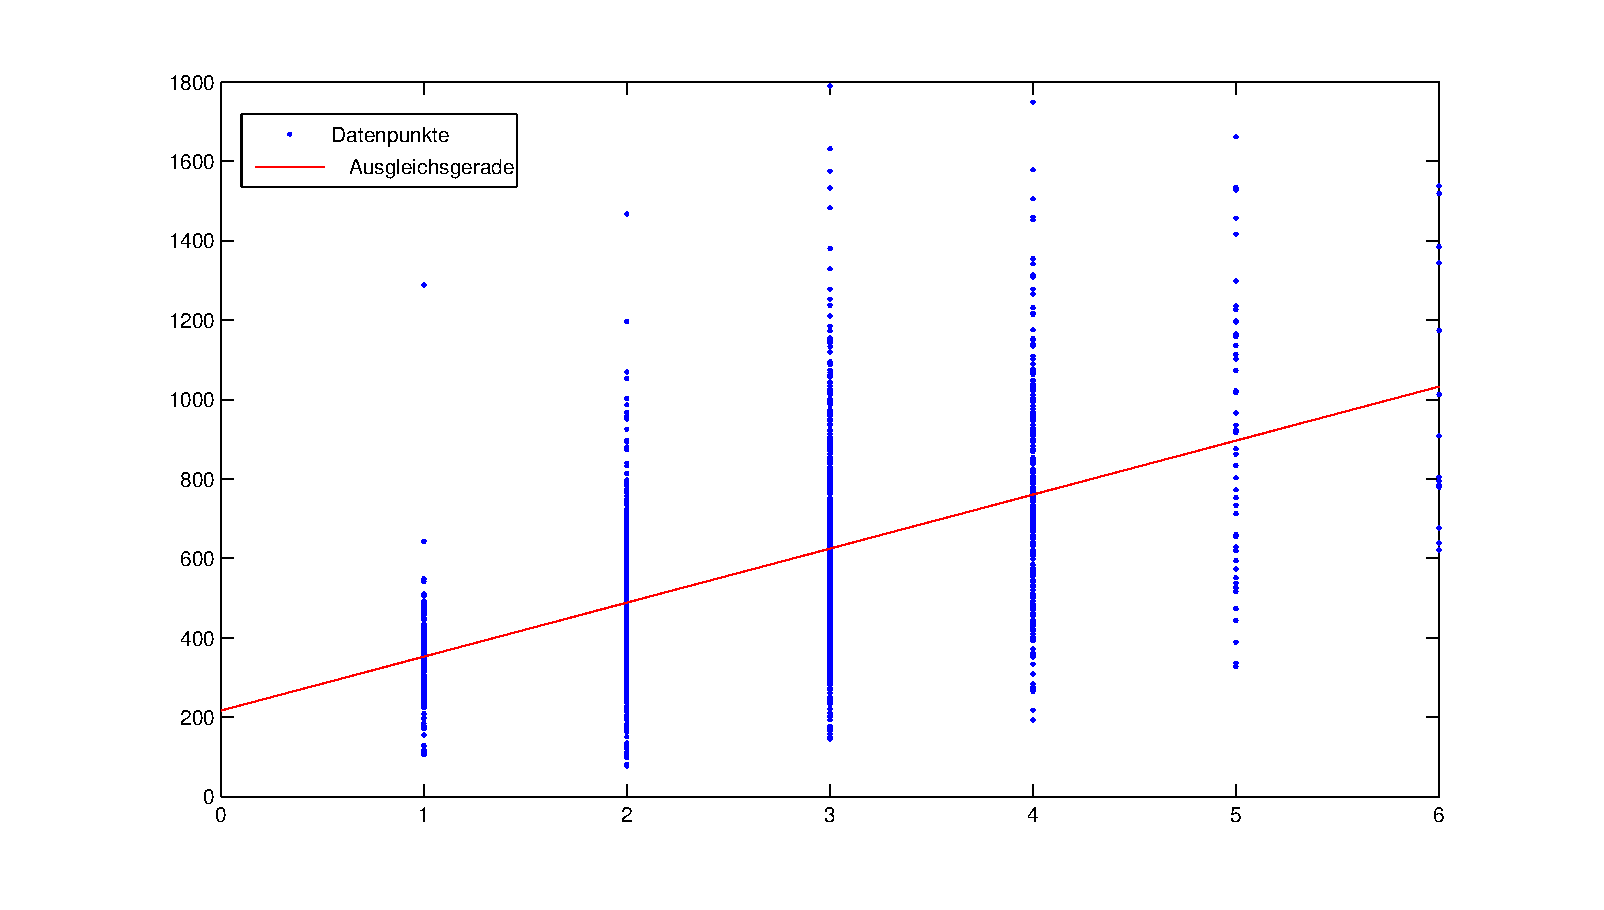
\includegraphics[width=0.8\textwidth]{figures/nm_rooms_distribution}
  \caption{Verteilung der Nettomieten in Abhängigkeit von der Raumanzahl mit der berechneten Ausgleichsgeraden. Datensatz: Münchener Mietspiegel 2003 \cite{Fahrmeir2011}.}
  \label{fig:nm_rooms_distribution}
\end{figure}
Ziel der Regression ist es nun, den Mietpreis als Funktion der Raumanzahl darzustellen:
\begin{equation*}
 M = f(R) + \epsilon ~.
\end{equation*}
Dabei ist $f$ eine beliebige Funktion und $\epsilon$ ein Fehlerterm.
Dieser wird benötigt, da die den Merkmalen zugehörigen Datensätze $(m_1, \dots, m_n)$, bzw. $(r_1, \dots, r_n)$ nie \textit{genau} auf der Regressionsgeraden liegen, sondern durch Messfehler oder nicht berücksichtigte Abhängigkeiten abweichen.
Der Erwartungswert für diese Fehler ist immer $0$. 
Um auch für kleinere Stichproben Aussagen über die Verteil"-ung der Schätzer machen zu können, wird meinst zusätzlich eine Normalverteilung angenommen \cite[S. 479]{Fahrmeir2010}:
\begin{equation*}
  E(\epsilon_i) = 0 \text{ und } \epsilon_i \sim N(0,\sigma^2), i = 1, \dots, n ~.
\end{equation*}
Diese Arbeit konzentriert sich nur auf lineare Funktionen $f$, aber in Abschnitt \ref{sec:mult_reg} wird gezeigt, wie auch ein logarithmischer Zusammenhang zwischen Regressand und Regressor miteinbezogen werden kann.
Hier ist aber ein linearer Zusammenhang naheliegend, daher wählen wir auch einen einfachen linearen Ansatz:
\begin{equation*}
  M = \alpha + \beta R + \epsilon ~.
\end{equation*}
Dieser Ansatz lässt sich natürlich auf beliebige Merkmale übertragen.
Um nun die Ausgleichsgerade wie in Abbildung \ref{fig:nm_rooms_distribution} zu erhalten, ist es nötig die Parameter $\alpha$ und $\beta$ so zu schätzen, dass der quadratische Fehler minimal wird.
Dieses Verfahren wird  \textit{Methode der kleinsten Quadrate} (KQ-Methode) genannt.
Formal sieht der Ansatz wie folgt aus:
\begin{equation*}
  \sum\limits_{i=1}^{n} \epsilon^2 = \sum\limits_{i=1}^{n} (m_i - \alpha - \beta r_i)^2 \rightarrow \min\limits_{\alpha, \beta} ~.
\end{equation*}
Die minimierenden Werte werden mit $\hat\alpha$ und $\hat\beta$ notiert und als \textit{Kleinste-Quadrate-Schätzer} bezeichnet.
Für unseren linearen Ansatz können beide Schätzer relativ einfach berechnet werden.
Der Regressionskoeffizient $\hat\beta$ ist allgemein für zwei Merkmale $X$ und $Y$ gegeben durch
\begin{equation*}
  \hat\beta = \frac{\tilde s_{XY}}{\tilde{s}^2_X} = \frac{\sum\limits_{i=1}^{n} y_i x_i - n \bar y \bar x}{\sum\limits_{i=1}^{n} x_i^2 - n \bar{x}^2} ~.
\end{equation*}
wobei $\tilde{s}^2_X$ die Varianz von $X$ und $\tilde s_{XY}$ die Kovarianz von $X$ und $Y$ bezeichnet. 
Wenn der Koeffizient bekannt ist, kann er in dir folgende Gleichung eingesetzt werden um die Konstante $\alpha$ zu erhalten:
\begin{equation*}
  \alpha = \bar y - \hat\beta \bar x ~.
\end{equation*}
Die Beweise für beide Rechnungen wurden hier aus Platzgründen ausgelassen, sind aber in \citet[S. 155]{Fahrmeir2010} zu finden.
% TODO: Muss der Durchschnitt hier erklärt werden?

Mithilfe dieser Methode erhalten wir nun die Schätzer für unser Beispiel.
Durch einfaches Einsetzen der Daten erhalten wir folgendes Ergebnis (Alle Zahlen wurden auf eine Stelle hinter dem Komma gerundet):
\begin{equation*}
  \hat\beta = \frac{\sum\limits_{i=1}^{n} m_i r_i - n \bar m \bar r}{\sum\limits_{i=1}^{n} r_i^2 - n \bar{r}^2}
  = \frac{3309500 - 2053 * 570.1 * 2.6}{15833 - 2053 * 2.6^2}
  \approx 136
\end{equation*}
\begin{equation*}
  \hat\alpha = \bar m - \hat\beta \bar r 
  = 570.1 - 136 * 2.6 
  \approx 216.8 ~.
\end{equation*}
Somit hat die Ausgleichsgerade in Abbildung \ref{fig:nm_rooms_distribution} die Gleichung $\hat m = 216.8 + 136 r$
Wir schreiben hier $\hat m$, da die Regressionsgerade eine Schätzung für die Nettomiete ist.

Die anfängliche Vermutung eines linearen Zusammenhangs zwischen der Anzahl der Zimmer und der Nettomiete ist damit bestätigt.
Man kann das Ergebnis weiterhin so interpretieren, dass es für jede Wohnung eine Grundmiete in Höhe von \EUR{216,80} gibt, die dann pro Zimmer um \EUR{136} erhöht wird.
Diese Interpretation ist allerdings in diesem Fall nicht unbedingt zielführend, da man schon mit bloßem Auge erkennen kann, dass die Residuen (Abweichungen der einzelnen Datenpunkte von der Ausgleichsgeraden) groß sind.
Daher wird die Annahme, wenn auch grundsätzlich richtig, wohl nur auf wenige Wohnungen zutreffen.
\\

Die Berechnung in der Funktion nag\_simple\_linear\_regression der \naglib erfolgt grundsätzlich wie oben beschrieben, allerdings mit einer Ausnahme: Es ist zusätzlich möglich die einzelnen Datenpunkte zu gewichten.
Dies führt dazu dass bei der Methode der kleinsten Quadrate auch die Fehler gewichtet eingehen, daher ist der Ansatz zur Minimierung dann $\sum\limits_{i=1}^{n}w_i\epsilon_i \rightarrow min$, wobei $w_i$ die Gewichtungen für die einzelnen Datenpunkte sind.
Für eine vollständige Beschreibung der Berechnungen mit Gewichtung sei der Leser auf \cite{nag:g02cac} verwiesen.

\subsubsection{Methodenaufruf}
\label{sec:sim_reg_anwendung}

Nach der Beschreibung der Berechnung der einfachen linearen Regression wollen wir nun auf die Anwendung mittels der Funktion nag\_simple\_linear\_regression eingehen.
Die Funktionsdeklaration ist in Listing \ref{lst:nag_simple_linear} zu sehen.
\begin{figure}[t]
  \begin{lstlisting}[caption={Deklaration der Methode \glqq nag\_simple\_linear\_regression\grqq, mit der eine einfache lineare Regression berechnet werden kann.}\label{lst:nag_simple_linear}, captionpos=b]
    void nag_simple_linear_regression (Nag_SumSquare mean, 
    Integer n, const double x[], const double y[], 
    const double wt[], double *a, double *b, double *a_serr, 
    double *b_serr, double *rsq, double *rss, double *df,
    NagError *fail)
  \end{lstlisting} 
\end{figure}
Es existieren insgesamt 13 Parameter, von denen die ersten Fünf Eingabe- und die Restlichen Ausgabeparameter sind.

Die wichtigsten Eingabeparameter sind die beobachteten Werte für das unabhängige(\lstinline{x[]}) und das abhängige(\lstinline{y[]}) Merkmal.
Für den Parameter \lstinline{n} muss nur die Anzahl der Beobachtungen angegeben und für \lstinline{wt[]} kann ein Array mit Gewichtungen für eingetragen werden.   
Falls keine Gewichtung gewünscht ist genügt es einen Null-Zeiger (zB. \lstinline{(double *) 0}) anzugeben.
Zuletzt existiert noch \lstinline{mean}.
Falls hier der Wert 'Nag\_AboutZero' angegeben wird, wird die Konstante $\alpha$ nicht in den Regressionsansatz miteinbezogen, d.h. die Regressionsgerade geht in jedem Fall durch den Ursprung.
Für die normale Berechnung kann 'Nag\_AboutMean' angegeben werden.

Die Ergebnisse der Regression $\hat\alpha$ und $\hat\beta$ sind nach Ausführung der Methode über die Zeiger \lstinline{*a} und \lstinline{*b} erreichbar.
Zudem werden auch einige Informationen zurückgegeben, die helfen die Güte des Regressionsansatzes zu überprüfen.
Da sind zunächst die Standartfehler \lstinline{*a_serr} und \lstinline{*b_serr}, die einen Hinweis darauf geben, wie genau die Koeffizienten geschätzt werden konnten.
Einen Hinweis auf die Güte des Regressionsmodells gibt das Bestimmtheitsmaß $R^2$ in \lstinline{*rsq}.
Es sagt aus, ein wie großer Anteil einer Variation des abhängigen Merkmals durch das unabhängige Merkmal erklärt wird.
Definiert ist es als Quadrat der Korrelation $R^2 = r_{XY}^2$ und nimmt daher Werte zwischen 0 und 1 an.
Ist der Wert niedrig, deutet dies auf ein schlechtes Regressionsmodell hin, da der Wert der abhängigen Variable dann stark von anderen, nicht beachteten, Einflüssen abhängig ist.
Zusätzlich wird noch die Summe der Fehlerquadrate (der minimierte Wert) in \lstinline{*rss} geschrieben.
Falls diese Summe sehr groß ist, weist das darauf hin, dass die Regressionsfunktion eine zu niedrige Komplexität haben könnte, um den Zusammenhang zwischen Regressor und Regressand hinreichend abzubilden.
Zuletzt gibt die Funktion über \lstinline{*fail} einen Fehler vom Typ \lstinline{NagError} aus, falls die Eingabeparameter falsch gesetzt wurde, oder das SVD Verfahren nicht konvergiert.

% TODO: Erwähnen, dass Beispielaufruf in Beispielprogramm verfügbar ist.

\begin{comment}
\begin{itemize}
 \item Nichtlineare Regression
 \begin{itemize}
  \item Für Sättigungskurven und Wachstumsverläufe
  \item Mögliche Funktionen: exp, $x^2$, sin
  \item Berechnung durch kleinste Quadrate Methode mittels Transformation möglich
 \end{itemize}

 \item Beispiel: Regression der Nettomiete nach Wohnfläche
 \begin{itemize}
  \item Streudiagramm zeigt steigende Abweichung $\Rightarrow$ Multiple Regression nötig!
 \end{itemize}
\end{itemize}

\subsubsection{Beispiel}


\end{comment}

\subsection{Multiple Lineare Regression}
\label{sec:mult_reg}

% TODO: Referenzen!

Im letzten Abschnitt haben wir behandelt, wie man mittels einfacher Regression die Werte eines abhängigen Merkmals auf Grundlage der Werte eines unabhängigen Merkmals schätzen kann.
Allerdings stößt die einfache Regression an Grenzen, wenn der Regressand von vielen Merkmalen beeinflusst wird, wobei die einzelnen Korrelationen an sich schwach sind.
Weiterhin bleiben offene Fragen: 
Wie verändert sich die Verteilung der Nettomieten zur Wohnfläche mit steigendem Baujahr?
Und wie groß ist der Einfluß von guter bzw. bester Wohnlage auf den Wohnungspreis? 
Diese können mit der multiplen linearen Regression gelöst werden, welche nun vorgestellt wird.

% Für die Berechnung über Matrizen wird \cite{Fahrmeir1984} für die theoretischen Grundlagen verwendet.
Die multiple Regression ist zunächst einmal eine Erweiterung der einfachen Regression auf eine beliebige Anzahl von Regressoren.
Dementsprechend wird auch das Regressionsmodell selbst auf $p$ unabhängige Merkmale erweitert:
\begin{equation*}
  Y_i = \beta_0 + \beta_1 x_{i1} + \dots + \beta_p x_{ip} + \epsilon_i, \quad i = 1, \dots, n ~.
\end{equation*}
Die Notation ist wie folgt:
Das abhängige Merkmal $Y$ ist in den Zufallsvariablen $Y_i, \dots, Y_n$ modeliert und $x_{1j}, \dots, x_{nj}$ sind jeweils die beobachteten Werte für die $j$ verschiedenen Regressoren.
Außerdem sind die Fehlerterme $\epsilon_1, \dots, \epsilon_j$ genauso modeliert wie in Sektion \ref{sec:sim_reg} und $\beta_0$ bis $\beta_n$ bezeichnen die Regressionskoeffizienten.
$\beta_0$ nimmt dabei die Rolle des konstanten Terms ein, den zuvor $\alpha$ innehatte.

Die Idee zur Berechnung der Koeffizienten ist die Selbe wie zuvor:
Wieder wird die kleinste Quadrate Methode verwendet und den quadratischen Fehler zu minimieren:
\begin{equation*}
  \label{eq:kq_mul}
  \sum\limits_{i=1}^{n} (Y_i - \beta_0 -\beta_1 x_1 - \dots - \beta_p x_{ip})^2 \rightarrow \min\limits_{\beta_0,\beta_1,\dots,\beta_n} ~.
\end{equation*}
Damit dieses Minimierungsproblem eine eindeutige Lösung $\hat\beta_0, \hat\beta_1, \dots, \hat\beta_p$ hat, müssen nach \citep[S.496]{Fahrmeir2010} die beiden folgenden Voraussetzungen erfüllt sein:
\begin{enumerate}
  \item Es müssen mindestens so viele Beobachtungen vorliegen, wie es Variablen im Regressionsansatz gibt. 
    Für gute Schätzungen sollte die Anzahl der Beobachtungen sogar deutlich größer sein.
  \item Die Merkmale müssen voneinander unabhängig sein, d.h. es darf nicht möglich sein eine Regressionsvariable als Linearkombination der anderen Variablen zu schreiben: $X_j \neq \sum\limits_{k\neq j} a_k X_k + b,~ \forall a_k, b$ muss gelten!
    Ist dies nicht der Fall ist mindestens eine der Variablen überflüssig, da mehrere den gleichen Anteil der Varianz des Regressanden erklären.  
\end{enumerate}

Auch wenn das Modell der multiplen linearen Regression nicht bedeutend komplexer als das der einfachen linearen Regression erscheint, so ist die Berechnung doch ungleich schwieriger.
So ist es jetzt nicht mehr möglich einfache direkte Formeln für die Berechnung der Regressionskoeffizienten anzugeben.
Stattdessen erfolgt die Berechnung nun mit Hilfe von Matrizen und Vektoren.
Als nächstes wollen wir zeigen wie genau die multiple Regression von der \naglib berechnet wird.
Auf die Demonstration der Berechnung anhand der Beispieldaten wird dabei verzichtet, allerdings wird das Ergebnis einer Regression in Sektion \ref{sec:reg_mul_ergebnis} vorgestellt und interpretiert.

\subsubsection{NAG Algorithmus}

In der NAG-Bibliothek wird die multiple Regression hauptsächlich durch die Funktion nag\_regsn\_mult\_linear zur Verfügung gestellt.
% TODO: KQ_Methode vorher definieren
Da die Berechnung wie bereits erwähnt mit Hilfe von Matrizen erfolgt, können wir den Minimierungsan"-satz der KQ-Methode wie folgt anpassen:
\begin{equation*}
  \label{eq:minimization}
  \sum\limits^{N}_{n=1} \epsilon^2_n = \epsilon^T \epsilon = (y - X \beta)^T (y - X \beta) \rightarrow \min\limits_{\beta} ~.
\end{equation*}
$\epsilon$ ist dabei der Vektor, der alle $\epsilon_i$ enthält und $X$ ist eine $n \times p$ Matrix mit den beobachteten Werten für alle Regressoren.
Außerdem sind $y$ und $\beta$ Vektoren, die beobachteten Werten für den Regressanden und die Koeffizienten beinhalten. 
Der erste Schritt ist dabei nur ein formales Umschreiben des KQ-Ansatzes durch Vektoren.
Anschließend werden die Fehlervektoren, durch ihre Definition, die Abweichung der berechneten Werte ($X\beta$) von den tatsächlichen Werten ($y$), ersetzt.
Da der Wurzel-Operator keinen Einfluß auf den Wert des Minimums hat, können wir die Forderung wie folgt umformulieren:
\begin{equation*}
  \label{eq:minimization_general}
  \Vert X\beta - y \Vert_2 \rightarrow \min\limits_{\beta} ~.
\end{equation*}
Um dieses Minimum zu erhalten, wird in nag\_regsn\_mult\_linear die QR-Zerlegung der Matrix $X$ berechnet.

Für die QR-Zerlegung gilt $X = QR$, wobei $Q$ eine orthogonale Matrix und $R$ eine obere rechte Dreiecksmatrix ist.
Die drei am meisten verbreiteten Verfahren zur Berechnung einer QR-Zerlegung sind folgende \citep[S. 211ff]{Golub1989}: Householder Transformationen, Givens Rotationen und das modifizierte Gram-Schmidt Verfahren.
Es ist nicht bekannt welches dieser Verfahren von der \naglib verwendet wird, allerdings sind nach \cite{Golub1989} sowohl das modifizierte Gram-Schmidt Verfahren (S.227), als auch die Givens Rotationen (S.228) langsamer als die Householder Transformationen, wenn es um die Lösung von Ausgleichsproblemen geht.
Für unsere Berechnung können wir uns nun einige Eigenschaften der Matrizen $Q$ und $R$ zunutze machen und den zu minimierenden Term erneut umschreiben:
\begin{equation*}
  \label{eq:orthogonal_transformation}
  \Vert X\beta - y \Vert_2 = \Vert Q^T X \beta - Q^T y \Vert_2 = \Vert R_1 \beta - c \Vert_2 + \Vert d \Vert_2 ~.
\end{equation*}
Im ersten Schritt kommt uns zugute, dass die 2-Norm bei orthogonaler Transformation den Wert erhält.
Daher können wir den Term mit $Q^T$ multiplizieren (die Orthogonalität wird beim Transponieren erhalten).
Eine weitere praktische Eigenschaft von orthogonalen Matrizen ist es, dass die transponierte Matrix zugleich die Inverse ist.
Daher folgt aus $X = QR_1$ sofort $Q^T X = R_1$.
Der Vektor $c$ ist einfach definiert als das Ergebnis der Operation $Q^T y$.
Die letzte Umformung gibt auch direkt den nach der Minimierung verbleibenden Restfehler in $\|d\|_2$ an, weswegen es nun möglich ist $\|R_1\beta - c\|_2 = 0$ zu verlangen.

Um nun die Werte für die Koeffizienten zu erhalten, muss das folgende Gleichungssystem gelöst werden:
\begin{equation*}
  R\hat\beta = c_1 ~.
\end{equation*}
Dabei gilt $R_1 = \begin{bmatrix} R \\ 0\end{bmatrix}$ ($R$ enthält nur die ersten $p$ Zeilen aus $R_1$) und $c_1$ ist ein Vektor mit den ersten $p$ Einträgen aus $c$. 
Da $R$ eine obere rechte Dreiecksmatrix ist, ist dies durch Rückwärtseinsetzen möglich.
Dies führt allerdings nur zu einem eindeutigen Ergebnis, falls $R$ vollen Rang hat.
Da diese Forderung aber äquivalent dazu ist, dass $X$ einen vollen Rang hat \citep[S. 225]{Golub1989}, können wir in unserem Anwendungsfall davon ausgehen, dass dies fast immer zutrifft, da die Zahl der Beobachtungen ohnehin immer größer sein sollte als die Zahl der einbezogenen Merkmale (und die Beobachtungen normalerweise verschieden sind).
Falls der Rang von $R$ dennoch nicht voll sein sollte, wird die Singulärwertzerlegung (SVD-Verfahren) angewandt um ein Ergebnis zu finden. 
Diese wird hier nicht vorgestellt, weitere Informationen können aber in \cite{nag:g02dac} und \citep[S. 239f]{Golub1989} gefunden werden.

\begin{comment}
\subsubsection{Singulärwertzerlegung}
Wie zuvor bereits erwähnt, wird die Singulärwertzerlegung in nag\_regsn\_mult\_linear nur angewandt, wenn der Rang der Matrix $R$ und damit auch der Rang von $X$ nicht voll ist.
Da die Zahl der Beobachtungen aber ohnehin immer größer sein sollte als die Zahl der einbezogenen Merkmale (und die Beobachtungen normalerweise verschieden sind), sollte dieser Fall bei normaler nicht allzu oft eintreten, weswegen wir die Singulärwertzerlegung hier nur kurz behandeln.  
\end{comment}

\subsubsection{Anwendung}
\label{sec:reg_mul_ergebnis}

Nun wollen wir zeigen, wie wir die multiple Regression am Beispiel des Mietspiegeldatensatzes nutzen können.
Um die Fragen vom Anfang dieses Abschnitts zu beantworten, wählen wir einen Regressionsansatz mit der Nettomiete ($NM$) als Regressanden und den unabhängigen Merkmalen Wohnfläche($W$), gute Wohnlage($gL$) und Baujahr($Bj$) als Regressoren.
In diesem Fall lohnt es sich einen Blick auf die Verteilung der Nettomieten zu werfen, bevor der Regressionsansatz festgelegt wird.
Diese Verteilung ist in Abbildung \ref{fig:nm_wfl_distributions:normal} in Abhängigkeit von der Wohnfläche zu sehen.
\begin{figure}[t]
  \centering
  \begin{narrow}{-0.2\textwidth}{0.2\textwidth}
    \subfloat[][Normale Skala]{
      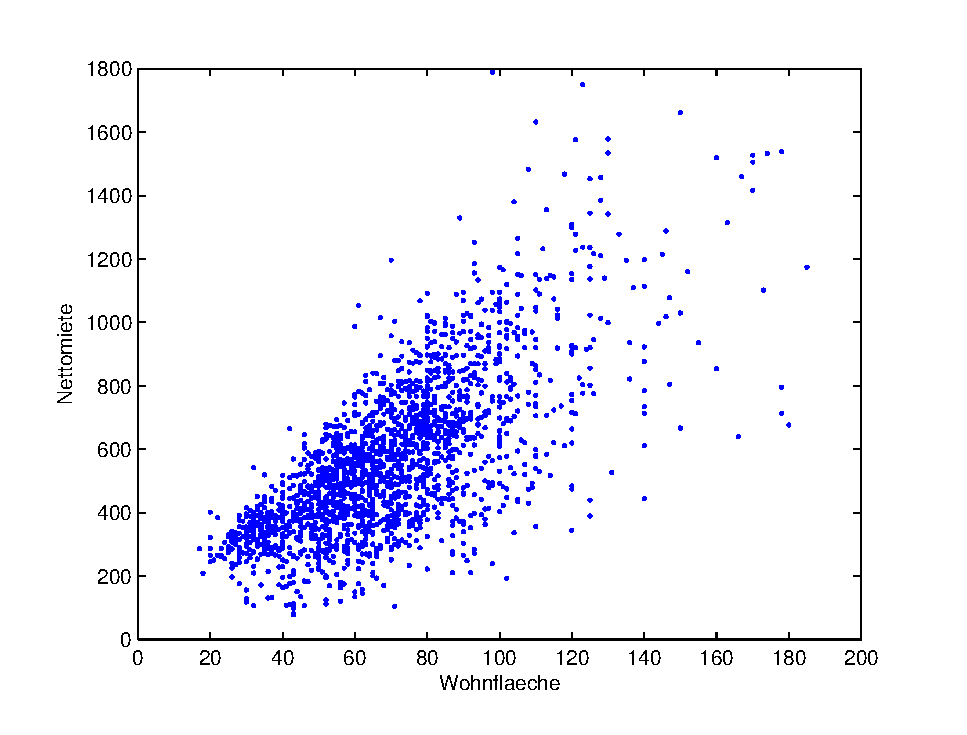
\includegraphics[width=0.7\textwidth]{figures/nm_wfl_distribution}
      \label{fig:nm_wfl_distributions:normal}
    }
    \subfloat[][Logarithmische Skala]{
      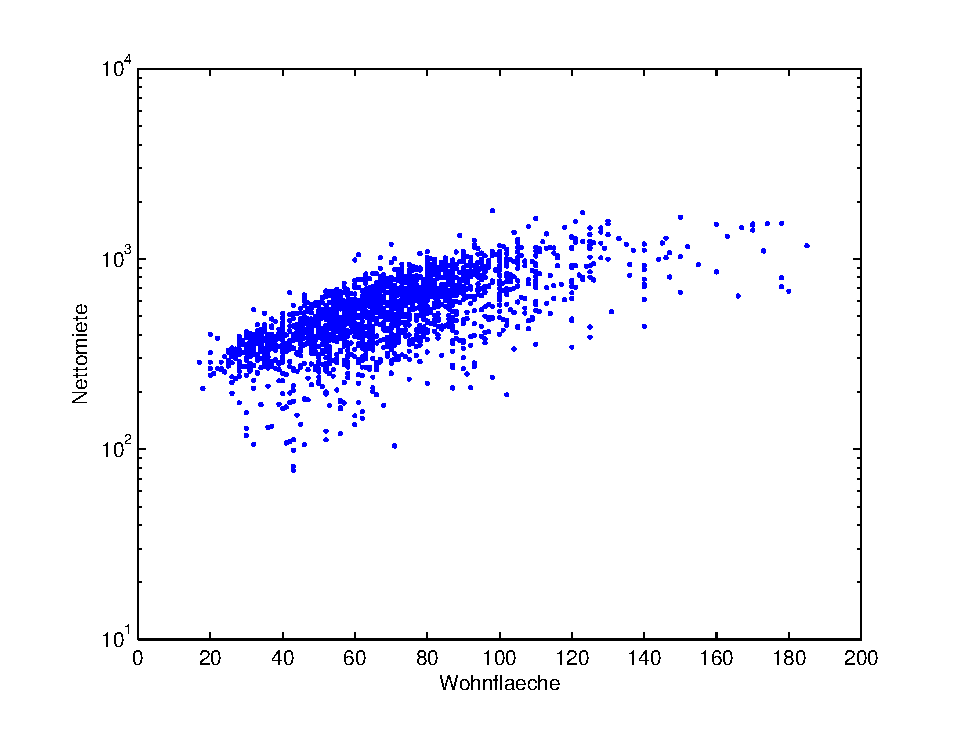
\includegraphics[width=0.7\textwidth]{figures/nm_wfl_distribution_log}
      \label{fig:nm_wfl_distributions:log}
    }
   
  \end{narrow}
  \caption{Die Verteilung der Nettomieten in Abhängigkeit von der Wohnfläche im Mietspiegel Datensatz.}
  \label{fig:nm_wfl_distributions}
\end{figure}
Es ist erkennbar, dass die Größe der Fehler mit steigender Wohnfläche zunimmt, was die Güte des Ergebnisses vermindert.
Eine bessere Verteilung ist mit einer logarithmischen Skala erkennbar (vgl. Abb. \ref{fig:nm_wfl_distributions:log}), weswegen wir $log(NM)$ anstelle von $NM$ als Zielvariable wählen:
\begin{equation*}
 log(NM) = \beta_0 + \beta_1 W + \beta_2 Bj + \beta_3 gL + \epsilon ~.
\end{equation*}

Unter Benutzung des zuvor vorgestellten Algorithmus erhalten wir folgenden Vektor mit den Regressionskoeffizienten:
\begin{equation*}
  \beta = \begin{pmatrix} \beta_0 \\ \beta_1 \\ \beta_2 \\ \beta_3 \end{pmatrix} = \begin{pmatrix} -2.83 \\ 0.01 \\ 0.004 \\ 0.11 \end{pmatrix}
\end{equation*}
Wenn diese Werte jetzt wieder in den Regressionansatz eingesetzt werden, erhalten wir das Ergebnis:
\begin{eqnarray*}
  \log(NM) & = & -2.83 + 0.01 W + 0.004 Bj + 0.11 gL + \epsilon\\
  \Rightarrow NM & = & \exp(-2.83) \exp(0.01 W) \exp(0.004 Bj) \exp(0.11 gL) ~.
\end{eqnarray*}
In der zweiten Zeile wurde der Regressionsansatz dabei wieder rücktransformiert, damit wir eine Aussage über die Nettomiete erhalten und nicht über ihren Logarithmus.

Da das Merkmal \glqq gute Wohnlage\grqq~ binär ist, können wir nun noch die Basismiete und den Aufpreis für eine Wohnung in guter Wohnlage bestimmen: $NM = NM_B \alpha$.
Die Basismiete $NM_B$ ergibt sich, wenn $gL$ auf 0 gesetzt wird:
\begin{equation*}
  NM_B = 0.059 \cdot \exp(0.012 W) \exp(0.004 Bj) ~.
\end{equation*}
Dieses Verhältnis zwischen Nettobasismiete, Wohnfläche und Baujahr ist in Abbildung \ref{fig:3d_result} geplottet.
\begin{figure}[t]
  \centering
  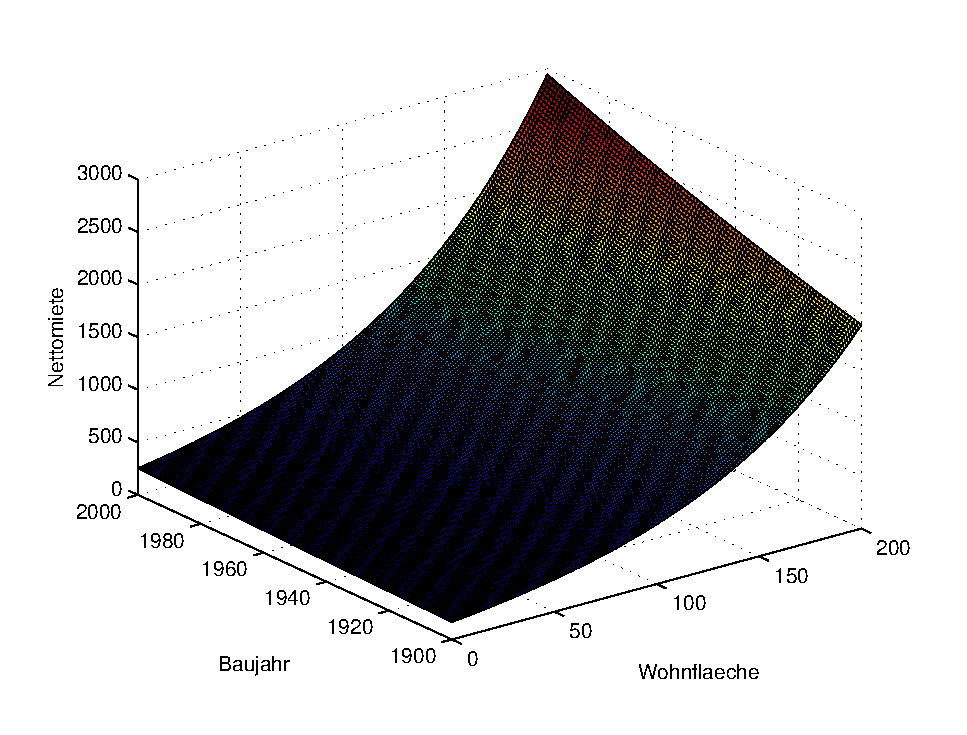
\includegraphics[width=10cm]{figures/nm_wfl_bj_log_approach}
  \caption{Das Ergebnis der Regression der Nettomiete mit den Regressanden Wohnfläche und Baujahr.}
  \label{fig:3d_result}
\end{figure}
Man kann erkennen, dass die Nettomiete sowohl mit zunehmendem Baujahr als auch mit zunehmender Wohnfläche ansteigt, was auch den Erwartungen entspricht.
Zusätzlich dazu kann man aber noch sehen, dass die Miete im Verhältnis zur Wohnfläche mit neuerem Baujahr immer schneller wächst, ein Ergebnis, das mit der einfachen Regression nicht hätte erreicht werden können.

Der Aufschlag für gute Wohnlage geht dann als Faktor in die Berechnung ein: $\alpha = exp(0.105) = 1.111$.
Für eine Wohnung in guter Wohnlage muss also mit einem Aufschlag von $11.1 \%$ auf die Basismiete gerechnet werden.


\subsubsection{Methodenaufruf}

Bei Benutzung der \naglib kann die multiple Regression durch die Funktion nag\_regsn\_mult\_linear berechnet werden.
Die Deklaration dieser Methode wird in Listing \ref{lst:nag_multiple_linear} gezeigt.
\begin{figure}[t]
\begin{lstlisting}[caption={Deklaration der Methode nag\_regsn\_mult\_linear, welche eine multiple lineare Regression ausführt.}\label{lst:nag_multiple_linear},captionpos=b]
void nag_regsn_mult_linear (Nag_IncludeMean mean, Integer n, 
    const double x[], Integer tdx, Integer m, 
    const Integer sx[], Integer ip, const double y[], 
    const double wt[], double *rss, double *df, double b[], 
    double se[], double cov[], double res[], double h[], 
    double q[], Integer tdq, Nag_Boolean *svd, Integer *rank, 
    double p[], double tol, double com_ar[], NagError *fail)
\end{lstlisting}
\end{figure}

Da die Methode sehr viele Parameter (24) hat, werden wir uns hier auf die Interessantesten beschränken.
Einige Parameter sind zudem äquivalent zu Parametern der Funktion nag\_simple\_linear\_regression, welche bereits in Sektion \ref{sec:sim_reg_anwendung} behandelt wurden und können auch genau so verwendet werden.
Diese sind: \lstinline{mean}, \lstinline{n}, \lstinline{x[]}, \lstinline{y[]}, \lstinline{wt[]}, \lstinline{*rss} und \lstinline{*fail}.
Für \lstinline{x[]} muss in diesem Fall verständlicherweise eine Matrix statt eines Vektors angegeben werden und die zulässigen Werte für \lstinline{mean} sind Nag\_MeanInclude (konstanten Term miteinbeziehen) und Nag\_MeanZero (kein konstanter Term).

Zu den genannten Parametern kommen weitere Eingabeparameter hinzu, mit denen die Regressoren aus den Merkmalen im Datensatz ausgewählt werden können.
Die Gesamtzahl an unabhängigen Variablen im Datensatz wird in \lstinline{m} gesetzt.
Im Vektor \lstinline{sx[]} der Länge $m$ wird dann für alle Regressoren ein Wert $>0$ eingetragen, alle anderen Felder erhalten eine Null.
Die Anzahl der Regressoren muss zusätzlich in \lstinline{ip} gegeben werden.
Für \lstinline{tol} muss zudem ein Toleranzwert angegeben werden, der bestimmt, wie groß der Unterschied zwischen zwei Zahlen sein darf, damit diese im Algorithmus noch als gleich groß behandelt werden. 
Das hat vor allem Auswirkungen auf den Rang der unabhängigen Variablen und beeinflusst damit, ob das SVD-Verfahren zum Einsatz kommt (Falls \lstinline{tol=0} verwendet wird ist dies nie der Fall).

Die Ausgabeparameter sind großteils von denen der einfachen Regressionsfunktion verschieden.
Am wichtigsten ist \lstinline{b[]}, welcher die berechneten Koeffizienten $\beta_0, \beta_1, \dots$ enthält.
Wie zuvor werden auch hier die zugehörigen Standartfehler in \lstinline{se[]} zurückgegeben.
Dazu kommen nun noch die Residuen für jede Beobachtung im Datensatz in \lstinline{res[]}, welche es einfach machen Ausreißer zu identifizieren.
Nach der Regression stehen außerdem Informationen zu den Verhältnissen der Regressoren untereinander in Form einer Kovarianzmatrix (\lstinline{cov}) zur Verfügung.
Diese enthält die Varianzen der Merkmale auf der Diagonalen und zudem alle möglich Kombinationen an Kovarianzen, was zum Beispiel ein schnelle Berechnung der Pearson-Korrelation ermöglicht (siehe auch Sektion \ref{sec:brav_pear_korr}).
Zuletzt geben \lstinline{*rank} und \lstinline{*svd} noch den Rang der Regressoren an und ob bei der Berechnung die Singulärwertzerlegung benutzt wurde.
\\

Zusätzlich zu nag\_regsn\_mult\_linear stellt die \naglib einige andere Funktionen zu Verfügung, die es ermöglichen das Regressionsmodell zu ändern, ohne die gesamte Regression erneut zu berechnen.
Diese Funktionen benötigen neben anderen Argumenten die QR-Zerlegung (welche von der Hauptfunktion als Zwischenergebnis in \lstinline{q[]} ausgegeben wird), die zugehörigen Informationen (\lstinline{p[]}) und die Beobachtungsmatrix $X$ und berechnen daraus aktualisierte Werte für die obere rechte Dreiecksmatrix $R$ und den Vektor $c$.
Im Gegensatz zu einer erneuten Berechnung mittels nag\_regsn\_mult\_linear hat dies den Vorteil, dass durch die Benutzung eines bereits bekannten Zwischenergebnisses Rechenzeit eingespart werden kann.
So kann der Benutzer beispielsweise mit nag\_regsn\_mult\_linear\_addrem\_obs neue Beobachtungen zum Modell hinzufügen oder sie entfernen.
Mit den Methoden nag\_regsn\_mult\_linear\_delete\_var und nag"-\_regsn\_mult\_linear\_add\_var werden aus dem Modell herausgenommen bzw. hinzu"-gefügt, wobei die Beobachtungen im letzteren Fall schon in $X$ enthalten sein sollten.
Zusätzlich dazu ist es auch noch möglich die abhängige Variable zu tauschen (nag\_regsn\_mult\_linear\_"-newyvar).

Nach Anwendung dieser Funktionen können die neuen Regressionskoeffizienten $\beta_0, \beta_1, \dots$ durch einen Aufruf von nag\_regsn\_mult\_linear\_upd\_model unter Angabe von $R$ und $c$ erhalten werden.
Die einzelnen Funktionen werden in dieser Arbeit nicht einzeln diskutiert, weitere Informationen sind aber unter \citep{nag:contents} verfügbar.






%\subsection{Analyse}

%TODO:Überarbeiten oder herausnehmen!
%Zusätzlich zu der Berechnung der verschieden Regressionsmodelle bietet die {\it NAG C Library} auch Funktionen zur Auswahl des Regressionsmodells und zur Modellvalidierung.

%Für die Auswahl des Modells sollen in der Arbeit zwei Metriken behandelt werden: Die Residualstreuung und das Bestimmtheitsmaß $\mathcal{R}^2$.
%Beide können uns eine Idee davon geben, wie gut die unabhängigen Variablen die Werte der abhängigen Variablen erklären können.
%Die Residualstreuung gibt die Verteilung der Differenzen zwischen der angenäherten Funktion und den wirklichen Daten an.
%Sollte sie unregelmäßig sein (wenn die Residuen beispielsweise mit einer Variablen anwachsen) ist dies ein starkes Indiz dafür, dass ein zu simples Modell gewählt wurde. 
%Das Bestimmtheitsmaß gibt dagegen an, wie gut abhängige Variable durch die Regression erklärt werden kann.
%Berechnet werden kann es auch durch eine Quadrierung des Bravais-Pearson Korrelationskoeffizienten, was den starken Zusammenhang von Korrelation und Regressionsanalyse zeigt.

%Für die Modellvalidierung stehen verschiedene Werkzeuge zur Verfügung, welche bei der Bewertung der Güte der Regression und deren Verbesserung genutzt werden können.
%In diese Kategorie fallen zum Beispiel der Cooks-Abstand (ermittelt besonders einflußreiche Punkte), die T-Statistik (Testet, ob eine unabhängige Variable für die Regression wichtig ist) oder der Durbin-Watson-Test (Ermittelt, ob die Residuen von den zuvor gemessenen Werten abhängig sind.
%In dieser Arbeit werden diese allerdings nicht weiter behandelt werden.

%%% Local Variables: 
%%% mode: latex
%%% TeX-master: "report"
%%% End: 

% LocalWords:  Raumanzahl


\section{Vergleich mit GNU Scientific Library}

In diesem Abschnitt werden wir die \naglib mit der {\it GNU Scientific Library} ({\it GSL}) vergleichen. Als Kriterien verwenden wir sowohl den jeweils gebotenen Funktionsumfang in den Bereichen Korrelation und Regression als auch die Leistung der entsprechenden Funktionen.

Die {\it GNU Scientific Library} ist eine unter der {\it GNU General Public License} ({\it GPL}) frei veröffentlichte numerische Bibliothek für {\it C} und {\it C++} \cite{GSL2011}. Zudem sind weitere Wrapper für andere Programmiersprachen ({\it Fortran}, {\it Perl}, {\it Python} etc.) sowie freie Erweiterungen erhältlich. Die Bibliothek bietet insgesamt über 1000 Funktionen, darunter auch zahlreiche für statistische Berechnungen, und wird unter anderem von {\it PSPP} genutzt, einer freien Alternative zur professionellen Statistik-Software {\it PASW Statistics} (ehemals {\it SPSS Statistics}).

\subsection{Funktionsumfang}
\label{sec:funktionsumfang}

Im Bereich der Korrelation gibt es zwischen der \naglib und der {\it GNU Scientific Library} wesentliche Unterschiede in der Funktionalität \cite{gsl:correlation}: Während erstere Funktionen zur Berechnung verschiedener Korrelationskoeffizienten und partieller Korrelation ({\it nag\_corr\_cov}, {\it nag\_ken\_spe\_corr\_coeff}, {\it nag\_partial\_corr}), zur Kovarianz ({\it nag\_sum\_sqs}, {\it nag\_sum\_sqs\_update}, {\it nag\_cov\_to\_corr}), zur robusten Korrelation ({\it nag\_robust\_}*) sowie zur Approximation ({\it nag\_nearest\_correlation}) anbietet, bietet letztere nur eine einzige Funktion ({\it gsl\_stats\_correlation}) an, mit welcher der Korrelationskoeffizient nach Bravais und Pearson berechnet werden kann. Eine Funktion zur Berechnung des Rangkorrelationskoeffizienten nach Spearman oder partieller Korrelation fehlt. Falls weitere Funktionen benötigt werden, müssen sie mit Hilfe anderer verfügbarer Funktionen zur Statistik selbst programmiert werden. Eine weitere Einschränkung der {\it GSL}-Funktion gegenüber der entsprechenden {\it NAG}-Funktion ({\it nag\_corr\_cov}) besteht darin, dass immer nur die Korrelation genau zweier Merkmale berechnet werden kann, die als Vektoren übergeben werden müssen. Als Ergebnis gibt die Funktion ausschließlich den berechneten Korrelationskoeffizienten in Form einer Gleitkommazahl zurück. Die {\it NAG}-Funktion zeigt sich wesentlich flexibler, ist es doch möglich, ihr eine Matrix mit zwei oder mehr Merkmalen zu übergeben, zu denen sie paarweise Korrelationskoeffizienten berechnet und wiederum in Form einer Matrix zurückgibt. Darüber hinaus gibt sie zusätzlich Zwischenberechnungen aus (siehe \refsec{sec:brav_pear_korr_funk}).

Insgesamt lässt sich also festhalten, dass die \naglib in diesem Bereich eine wesentlich größere Anzahl Funktionen bietet als die {\it GNU Scientific Library}, welche sich außerdem durch eine größere Flexibilität auszeichnen.

Auch im Bereich der Regression gibt es große Unterschiede in der Funktionalität.
Die in dieser Arbeit behandelten Regressionsarten finden sich aber in beiden Bibliotheken.
Während die einfache Regression in der \naglib von der Funktion nag\_simple\_linear\_regression berechnet wird, existieren in der GSL mehrere Funktionen zu diesem Zweck.
Diese sind gsl\_fit\_linear, für eine Regression mit konstantem Term, gsl\_fit\_wlinear für gewichtete Beobachtungen, sowie gsl\_fit\_mul bzw. gsl\_fit\_wmul für Regressionen ohne konstanten Term.

Ähnlich verhält es sich mit der multiplen Regression.
Hier stehen den beiden NAG Funktionen nag\_regsn\_mult\_linear und nag\_regress\_confid\_interval (für Konfidenzintervalle) die Funktionen  gsl\_multifit\_linear, gsl\_multifit\_wlinear und gsl\_multifit\_linear\_residuals (Berechnung der Residuen) gegenüber.
Zusätzlich ist es bei Benutzung der GSL möglich mit den Funktionen gsl\_multifit\_linear\_svd und gsl\_multifit\_usvd Einfluss auf die Berechnung der Singulärwertzerlegung zu nehmen, welche in der GSL zur Berechnung der Koeffizienten verwendet wird.
Die Dokumentation aller GSL Funktionen zur Regression ist unter \cite{FreeSoftwareFoundation2011} verfügbar.
Damit ist die Funktionalität der GSL allerdings auch erschöpft, während in der \naglib noch weitere Funktionalität zur Verfügung steht.

Eine weitere Möglichkeit der \naglib ist es, vorhandene Berechnungen wiederzuverwenden.
Mit Funktionen wie nag\_regsn\_mult\_linear\_add\_var, nag\_regsn\_mult\_linear\_delete\_var oder nag\_regsn\_mult\_linear\_addrem\_obs können Variablen oder Beobachtungen zum Modell hinzugefügt oder gelöscht werden.
Eine Aktualisierung der Koeffizienten erfolgt dann mit nag\_regsn\_mult\_"-linear\_"-upd\_model.
Es muss allerdings gesagt werden, dass diese Methode nicht immer zum gleichen Ergebnis führt wie die direkte Berechnung.
Stattdessen werden die bereits berechneten Koeffizienten nur minimal verändert und der neue Koeffizient wird so gewählt, dass die Residuen minimal sind. 

Außerdem werden auch Methoden angeboten, welche die Bestimmung des Regressionsmodells vereinfachen.
So berechnet die Funktion nag\_"-all\_"-regsn beispiel"-sweise die Quadratsumme der Residuen aller möglichen Regressionen für eine Menge von unabhängigen Variablen.
Weiterhin ist es möglich andere Verteilungen als die Normalverteilung für die Fehlerterme anzunehmen (zB. nag\_"-glm\_"-binomial).
Zuletzt existieren hier auch Funktionen für spezialisiertere Regressionsarten, wie zum Beispiel die robuste Regression oder die Ridge-Regression.

\subsection{Leistungsanalyse}
\label{sec:leistungsanalyse}

Die Leistungsanalyse wurde auf dem Rechner-Cluster der {\it RWTH Aachen} durch"-geführt. Es wurde ein System aus 9 {\it Sun Fire X4450}-Teilsystemen verwendet, welche jeweils über 4 {\it Xeon X7450}-Prozessoren mit 6 Kernen, eine Taktfrequenz von 2,66 GHz und x64-Architektur verfügten. Insgesamt standen somit 36 Prozessoren bzw. 216 Kerne sowie 128 GByte Arbeitsspeicher zur Verfügung. Es ist allerdings anzumerken, dass die Testprogramme nicht parallel programmiert wurden. Als Betriebssystem wurde {\it Linux} ({\it CentOS 5.6}) eingesetzt. Die Testprogramme wurden mit dem {\it Intel C++ 64 Compiler} ({\it ICC}) {\it 11.1} und aktivierter Optimierungsstufe O2 kompiliert, um Vergleichbarkeit der einzelnen Tests zu gewährleisten. Sonstige individuelle Optionen wurden nicht gesetzt.

Im Anhang dieser Arbeit sind exemplarisch die Quellcodes jeweils zweier Testprogramme zu Korrelation und Regression zu finden. Die übrigen Testprogramme sind analog aufgebaut und werden daher nicht alle aufgeführt.

% Graphik mit allen Kurven (Korrelation):
\begin{figure}[h]
  \centering
  \begin{narrow}{-0.2\textwidth}{0.2\textwidth}
    \subfloat[][Dauer der Berechnung des Bravais-Pearson-Korrelationskoeffizienten mit NAG und GSL (Zufallsdatensatz)]{
      \label{fig:analysis:test_corr_1_random}
      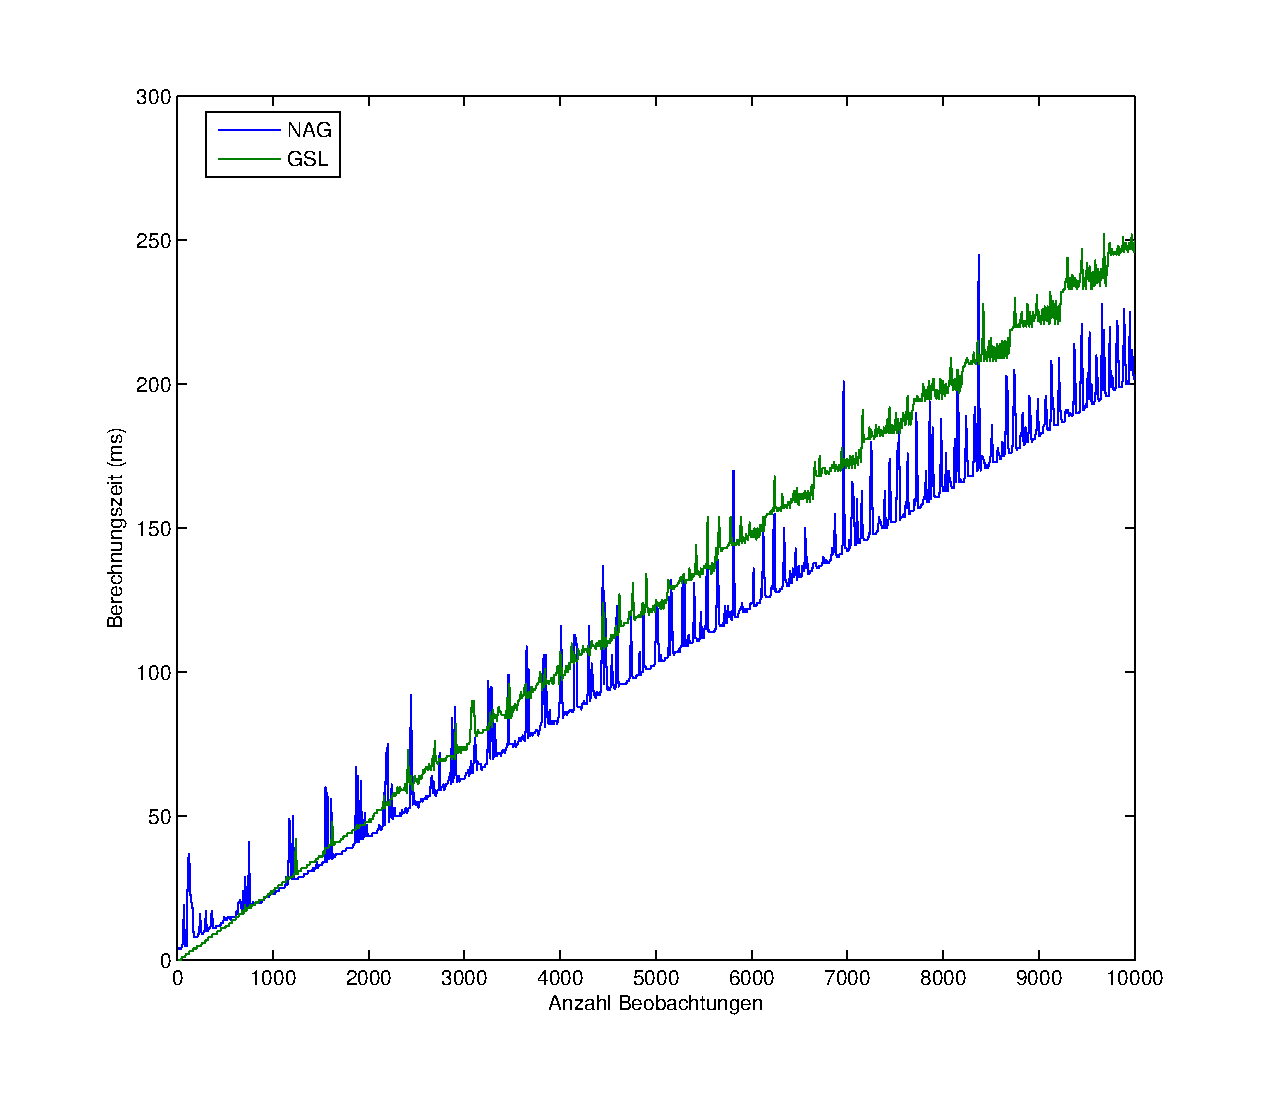
\includegraphics[width=0.6\textwidth]{figures/test_corr_1_random}
    }
    \subfloat[][Dauer der Berechnung des Bravais-Pearson-Korrelationskoeffizienten mit NAG und GSL (Münchener Mietspiegel 2003 \cite{Fahrmeir2011})]{
      \label{fig:analysis:test_corr_1_rent}
      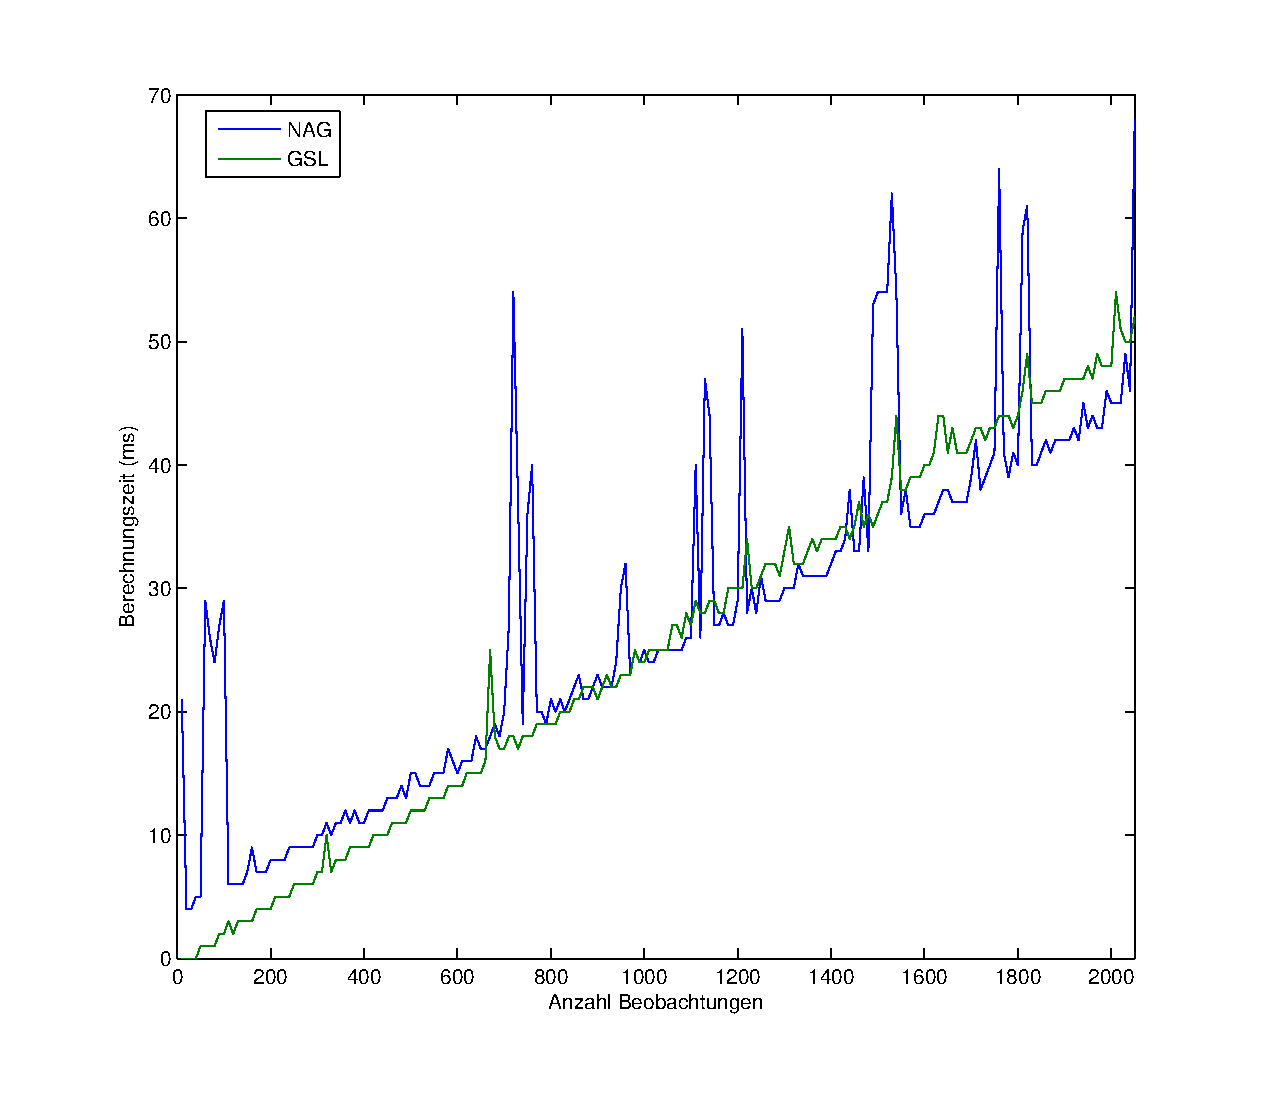
\includegraphics[width=0.6\textwidth]{figures/test_corr_1_rent}
    }\\
    \subfloat[][Dauer der Berechnung des Bravais-Pearson-Korrelationskoeffizienten und des Spearman-Rangkorrelationskoeffizienten mit NAG (Zufallsdatensatz)]{
      \label{fig:analysis:test_corr_2_random}
      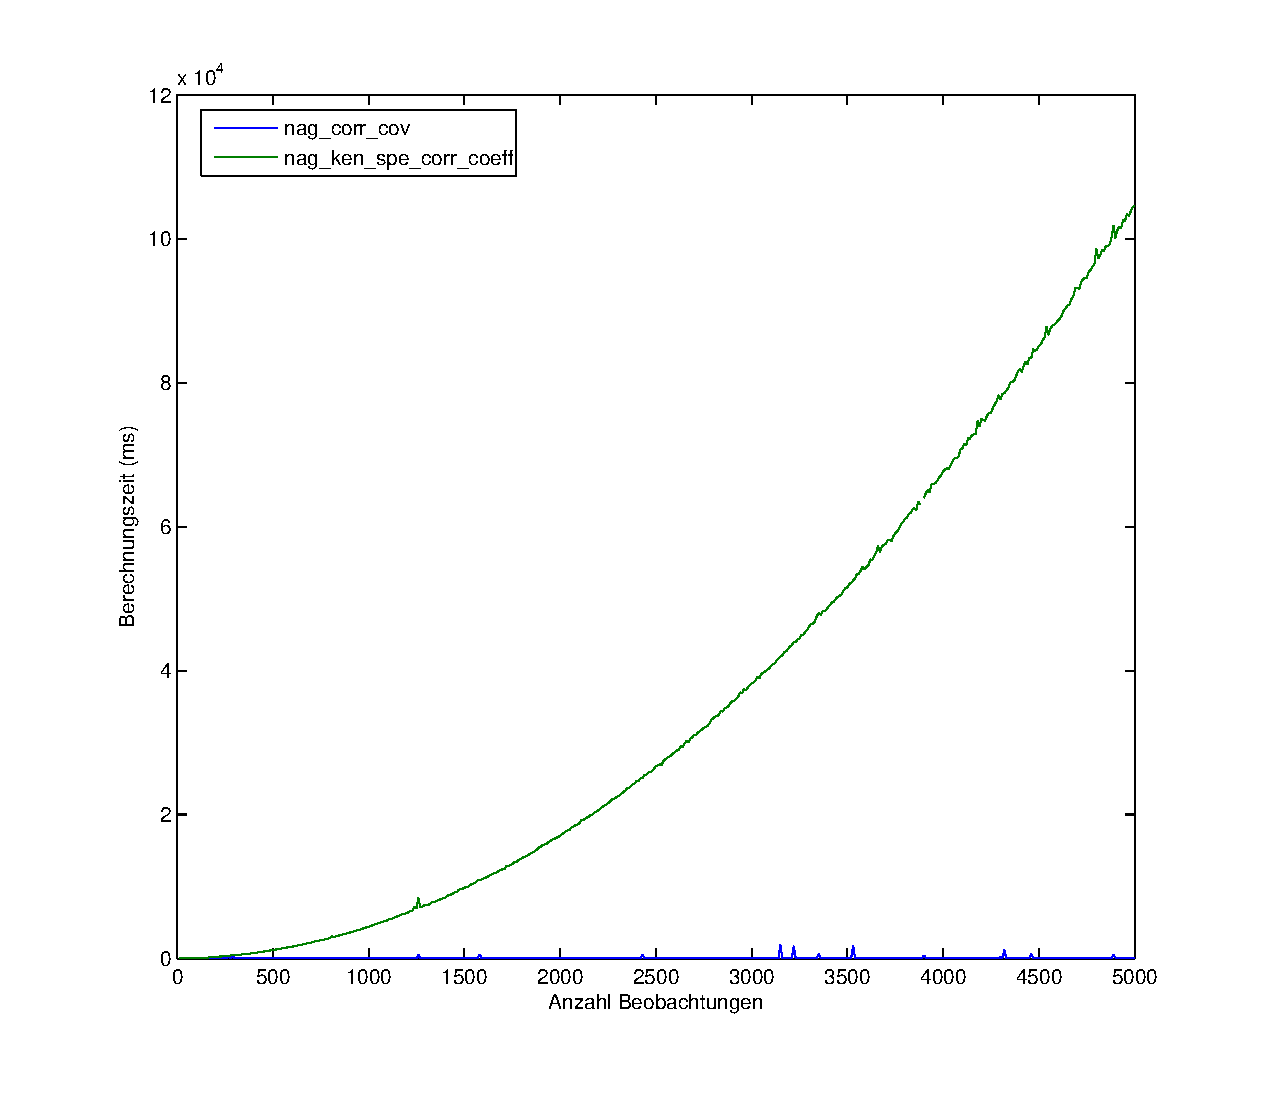
\includegraphics[width=0.6\textwidth]{figures/test_corr_2_random}
    }
    \subfloat[][Dauer der Berechnung des Bravais-Pearson-Korrelationskoeffizienten und des Spearman-Rangkorrelationskoeffizienten mit NAG (Münchener Mietspiegel 2003 \cite{Fahrmeir2011})]{
      \label{fig:analysis:test_corr_2_rent}
      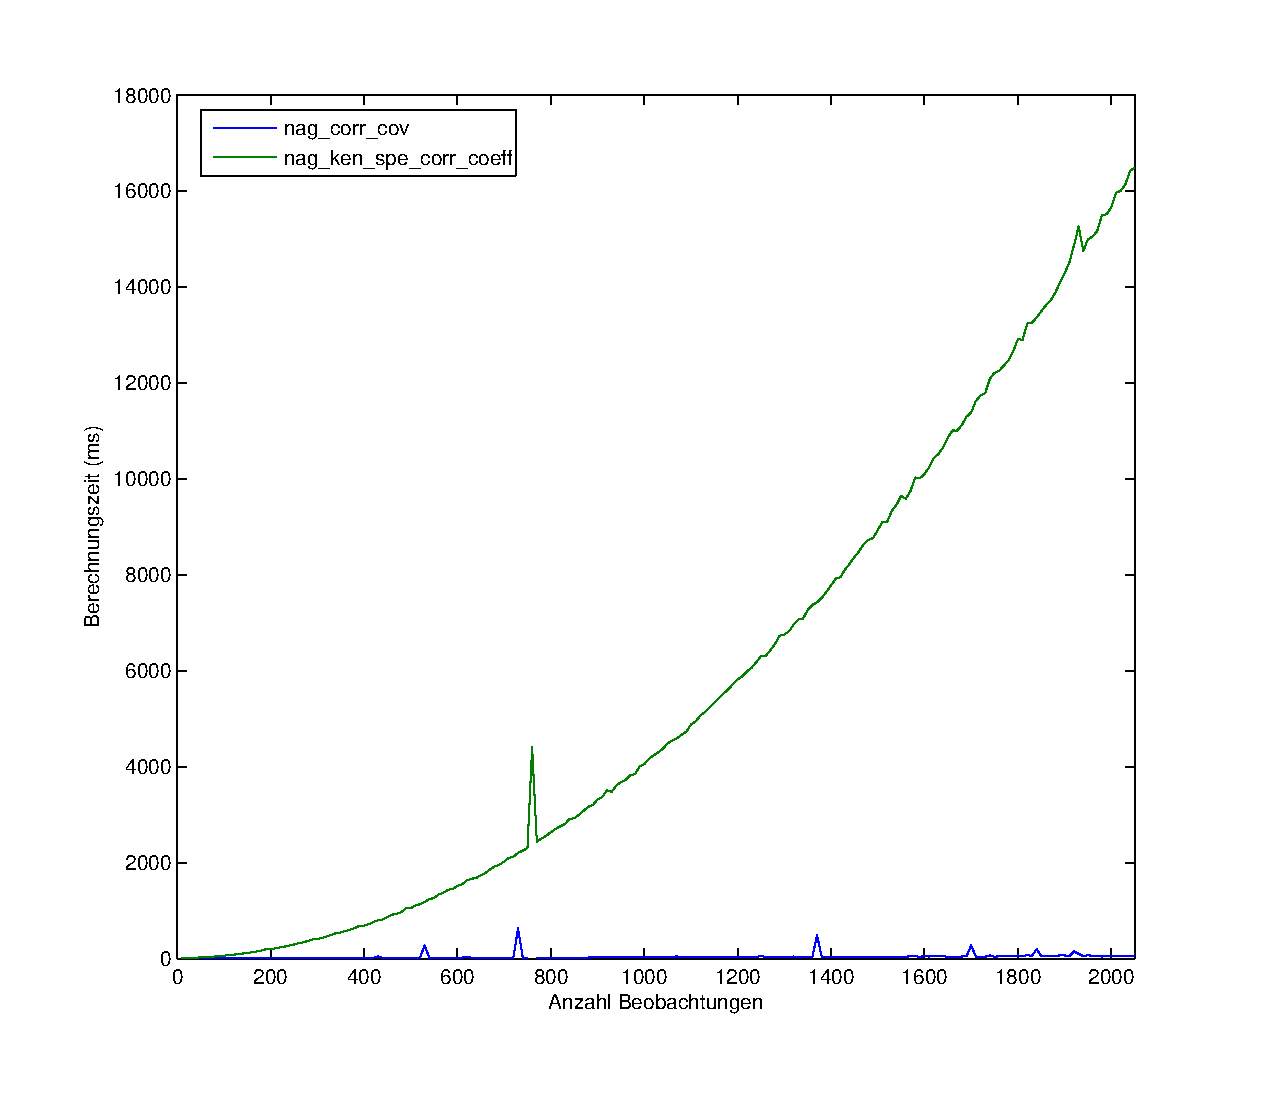
\includegraphics[width=0.6\textwidth]{figures/test_corr_2_rent}
    }\\
  \end{narrow}
  \caption{Ergebnisse der Leistungsanalyse zur Korrelation}
  \label{fig:analysis:correlation}
\end{figure}

% Graphik mit allen Kurven (Regression):
\begin{figure}[h]
  \centering
  \begin{narrow}{-0.2\textwidth}{0.2\textwidth}
    \subfloat[][Dauer der einfachen linearen Regression von NAG und GSL mit zunehmenden Beobachtungen aus dem Mietspiegeldatensatz\cite{Fahrmeir2011}.]{
      \label{fig:analysis:sim_reg_rent}
      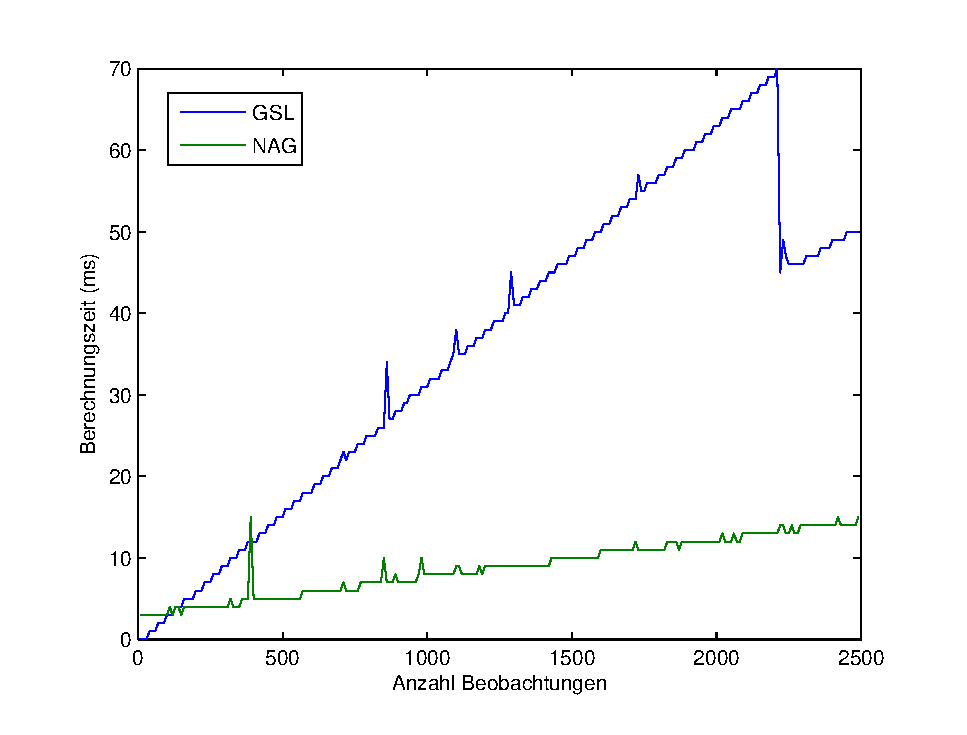
\includegraphics[width=0.6\textwidth]{figures/simple_reg_comp_rent}
    }
    \subfloat[][Dauer der einfachen linearen Regression von NAG und GSL mit zufälligen Daten.]{
      \label{fig:analysis:sim_reg_rand}
      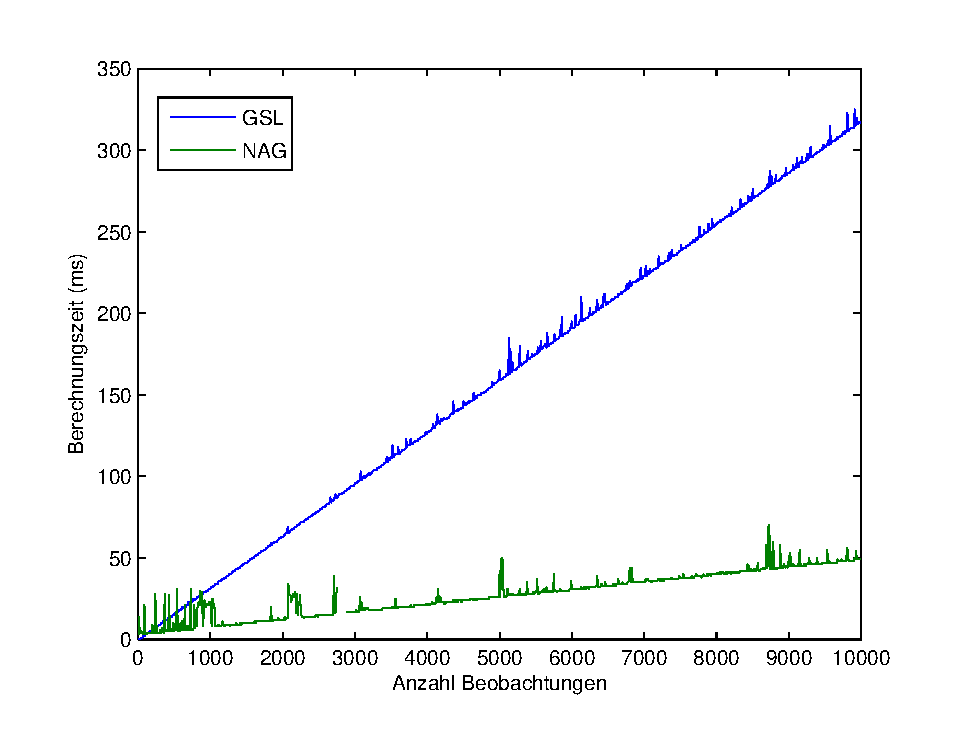
\includegraphics[width=0.6\textwidth]{figures/simple_reg_comp}
    }\\
    \subfloat[][Dauer der multiplen Regression von NAG und GSL mit 6 Merkmalen und zufälligen Daten.]{
      \label{fig:analysis:mul_reg_obs}
      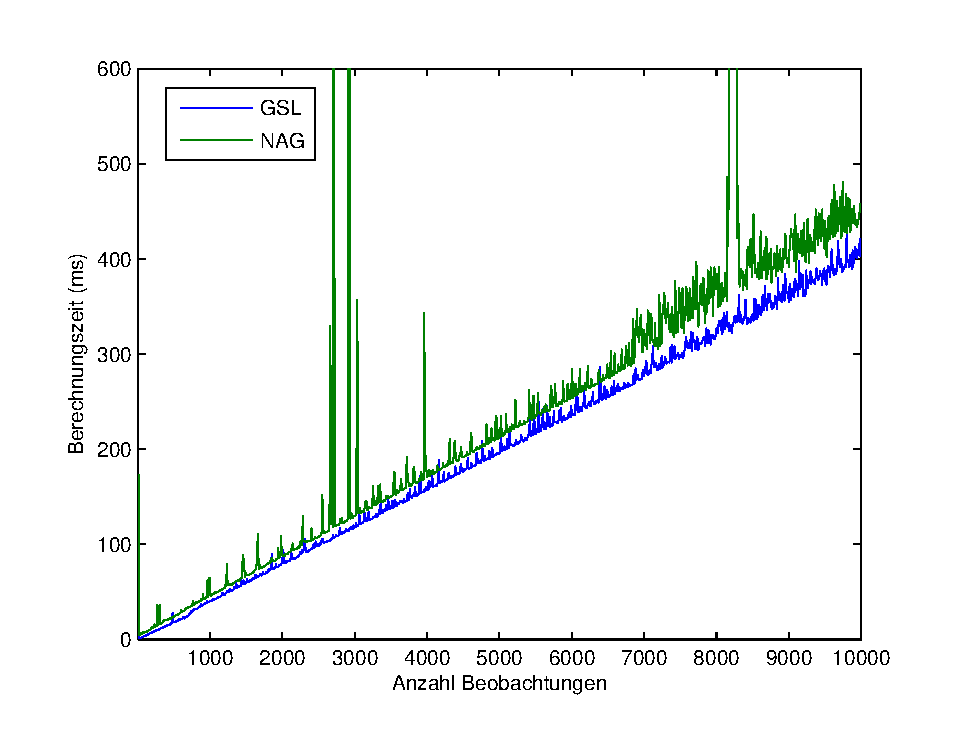
\includegraphics[width=0.6\textwidth]{figures/multi_reg_comp_6_var}
    }
    \subfloat[][Dauer der multiplen Regression von NAG und GSL mit 2500 Beobachtungen und zufälligen Daten.]{
      \label{fig:analysis:mul_reg_vars}
      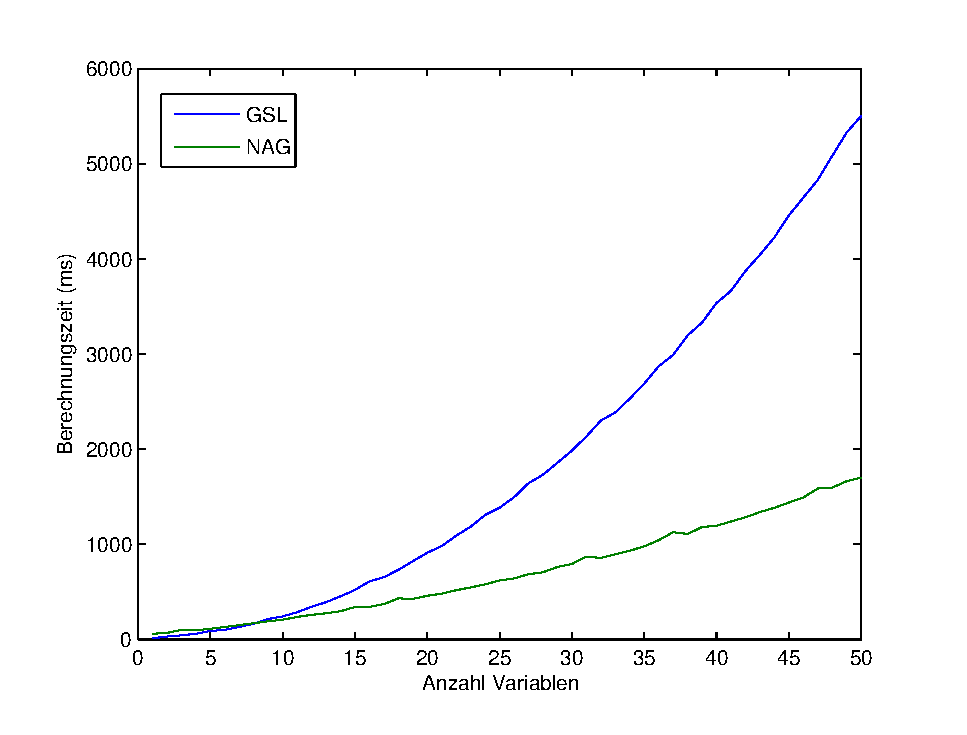
\includegraphics[width=0.6\textwidth]{figures/multi_reg_vars_2500_obs_rand}
    }\\
    \subfloat[][Unterschied zwischen direkter Berechnung und Aktualisierung mit Daten aus dem  Mietspiegeldatensatz\cite{Fahrmeir2011}.]{
      \label{fig:analysis:mul_reg_rent_act}
      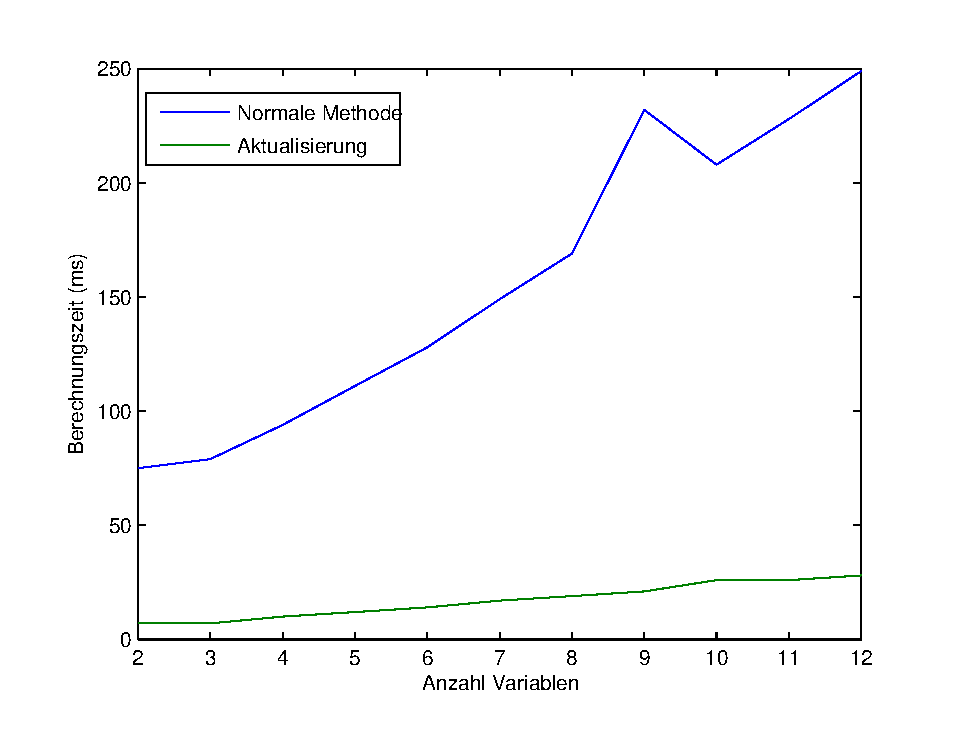
\includegraphics[width=0.6\textwidth]{figures/multi_reg_vars_2500_obs_act}
    }
    \subfloat[][Unterschied zwischen direkter Berechnung und Aktualisierung mit zufälligen Daten]{
      \label{fig:analysis:mul_reg_rand_act}
      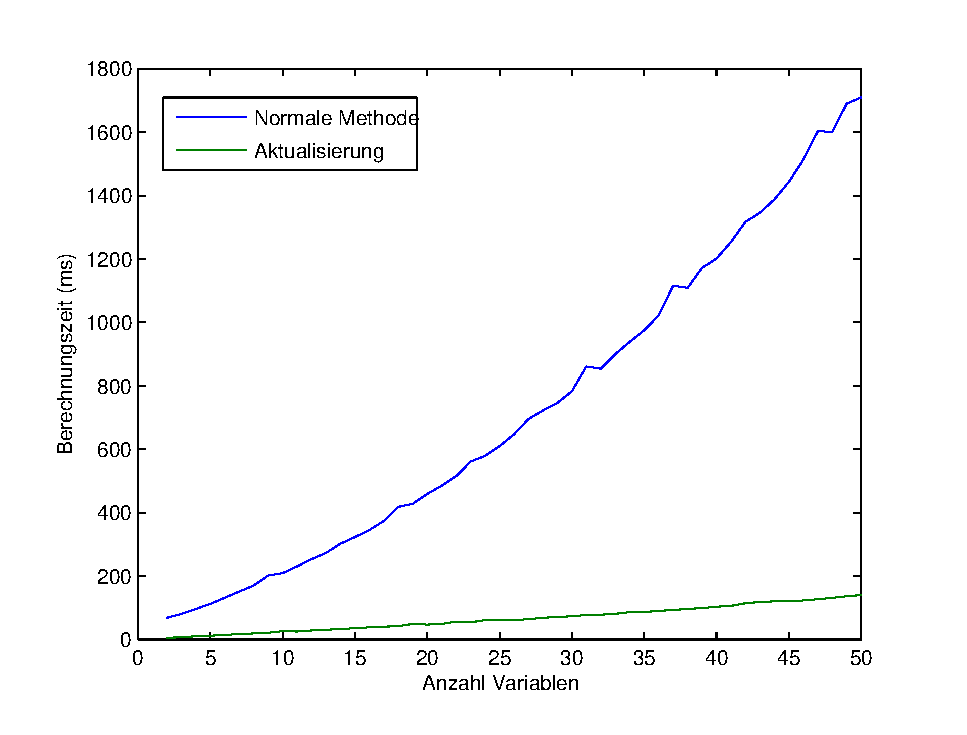
\includegraphics[width=0.6\textwidth]{figures/multi_reg_vars_2500_obs_act_rand}
    }
  \end{narrow}
  \caption{Ergebnisse der Leistungsanalyse zur Regression}
  \label{fig:analysis:regression}
\end{figure}

Hinsichtlich der Korrelation wurden zwei Tests durchgeführt: Im ersten Test wurde die {\it NAG}-Funktion zur Berechnung des Korrelationskoeffizienten nach Bravais und Pearson ({\it nag\_corr\_cov}) mit ihrem {\it GSL}-Pendant ({\it gsl\_stats\_correlation}) verglichen. Im zweiten Test wurden innerhalb der\naglib die Funktion zur Berechnung des Korrelationskoeffizienten nach Bravais und Pearson sowie jene zur Berechnung des Rangkorrelationskoeffizienten nach Spearman verglichen.

Der Testaufbau war in beiden Fällen gleich: Die verglichenen Funktionen erhielten pro Durchgang als Eingabe jeweils zwei Merkmale aus einem Zufallsdatensatz sowie anschließend aus dem {\it Münchener Mietspiegel 2003} \cite{Fahrmeir2011}. Während eines Durchgangs wurde die Anzahl der Beobachtungen schrittweise von 10 auf 10000 (Zufallsdatensatz) bzw. 2050 ({\it Münchener Mietspiegel 2003}) erhöht. Die Schrittweite betrug dabei 10. In jedem Schritt wurde die jeweilige Funktion 1000 mal berechnet und die gesamte Berechnungszeit gemessen.

Die Ergebnisse des ersten Tests sind in \reffig{fig:analysis:test_corr_1_random} und \reffig{fig:analysis:test_corr_1_rent} zu sehen. Wie gut ersichtlich ist, zeigen beide Funktionen ein lineares Wachstum, wobei die Berechnungszeit der {\it GSL}-Funktion bis zu etwa 900 Beobachtungen geringer als die der {\it NAG}-Funktion ist. Diese zeigt sich jedoch für jede größere Anzahl Beobachtungen im Durchschnitt (d.h. unter Relativierung der sichtbaren Schwankungen der Berechnungszeit) als geeigneter: Bei einer Anzahl von 10000 Beobachtungen braucht sie bereits etwa 45 ms weniger. Eine Empfehlung zur Verwendung der beiden Funktionen könnte daher lauten, erstere nur für kleine Datensätze zu verwenden und letztere für größere Datensätze ab etwa 900 Beobachtungen. Insgesamt hat hier also die {\it NAG}-Funktion die Nase vorn.

Die Ergebnisse des zweiten Tests können in \reffig{fig:analysis:test_corr_1_random} und \reffig{fig:analysis:test_corr_1_rent} abgelesen werden. Hier ist deutlich erkennbar, dass die Funktion zur Berechnung des Korrelationskoeffizienten nach Bravais und Pearson wesentlich schneller ist als jene zur Berechnung des Rangkorrelationskoeffizienten nach Spearman. Dies ist vermutlich durch die Berechnung der Ränge zu erklären, welche letztere Funktion zusätzlich leisten muss: Wenn man bedenkt, dass zur Rangbildung alle Beobachtungen zuerst nach ihren Messwerten sortiert werden müssen (siehe \refsec{sec:spear_rangkorr}) und es bekanntermaßen bisher keinen Sortieralgorithmus mit einer Worst-Case-Laufzeit von weniger als $\mathcal{O}(n \log{n})$ gibt. Eine Empfehlung ist daher, letztere Funktion wirklich nur dann einzusetzen, wenn sie zur Berechnung der Korrelation von ordinalskalierten Merkmalen unbedingt benötigt wird.

Für die Regression werden jeweils die Funktionen für die einfache und multiple lineare Regression der \naglib mit den Funktionen der GSL verglichen.
In Abbildung \ref{fig:analysis:sim_reg_rent} sind die Berechnungszeiten der Funktionen nag\_simple"-\_linear\_regression und gsl\_fit\_linear bei steigender Beobachtungszahl und unter Benutzung der Daten des Münchener Mietspiegels gezeigt.
Die angegebenen Zeiten entsprechen dabei jeweils 1000 Berechnungen.
Es ist zu erkennen, dass die NAG Funktion weit besser skaliert und bei 2500 Beobachtungen um den Faktor 3-4 schneller ist.
Dabei ist aber zu berücksichtigen, dass bei der NAG Funktion zusätzlich zum Regressionskoeffizienten und der Quadratsumme der Residuen noch und das Bestimmtheitsmaß und den Standardfehler berechnet, während die GSL Funktion zusätzlich die Kovarianzen der Koeffizienten zurück gibt.
Der Einbruch der Berechnungszeiten bei 2200 Beobachtungen ist reproduzierbar und tritt nur bei diesem Datensatz auf.
Der erkennbare Trend wird durch einen Vergleich mit zufälligen Daten und mehr Beobachtungen noch verstärkt (vgl. Abbildung \ref{fig:analysis:sim_reg_rand}).

Für den Vergleich der Leistungsfähigkeit bei der Berechnung der multiplen linearen Regression wurden zwei verschiedene Setups gewählt.
Zum einen wird wieder sukzessive die Anzahl der Beobachtungen erhöht zum anderen ist die Zahl der Regressoren variabel. 
Für beide Ansätze werden zufällige Daten benutzt, da die Anzahl der Beobachtungen und der Variablen hier nicht limitiert sind.
% TODO: Nummer des Anhangs einfügen
Da die Funktionen, wie auch bei der einfachen Regression, wieder nicht die gleichen Resultate zurück liefern, wurde bei der GSL Funktion zusätzlich das Bestimmtheitsmaß und die Residuen berechnet, um einigermaßen vergleichbare Daten zu erhalten.
Die Ergebnisse bei variablen Beobachtungen und sechs Regressoren sind in Abbildung \ref{fig:analysis:mul_reg_obs} zu sehen.
Die beiden Bibliotheken liegen hier fast gleichauf, wobei sich leichte Vorteile für die GSL zeigen.
Abbildung \ref{fig:analysis:mul_reg_vars} zeigt die Ergebnisse bei einer steigender Anzahl an Variablen bei 2500 Beobachtungen.
Auch hier liegt die GSL bei wenigen Regressoren vorne, ab neun Regressoren ist allerdings die NAG Funktion effizienter, welche auch bei weiter steigender Regressorenzahl besser skaliert.
Natürlich ist dabei zu bedenken, dass in den meisten Anwendungen wahrscheinlich nicht mehr als zehn Regressoren verwendet werden.

Außerdem haben wir noch die Geschwindigkeit der Methoden zur Aktualisierung eines Modells mit der der Neuberechnung in der \naglib verglichen.
Als veränderbaren Faktor benutzen wir hier wieder die Anzahl der Regressoren bei 100 Iterationen.
Es ist sowohl bei der Verwendung der Mietdaten (Abbildung \ref{fig:analysis:mul_reg_rent_act}), als auch bei der Verwendung von zufälligen Daten (Abbildung \ref{fig:analysis:mul_reg_rand_act}) zu erkennen, dass die Aktualisierungsmethode besser skaliert und um eine Faktor von 8 oder mehr schneller ist.
Dabei muss allerdings, wie schon zuvor erwähnt, berücksichtigt werden, dass die Regressionsergebnisse nicht äquivalent sind.

%%% Local Variables: 
%%% mode: latex
%%% TeX-master: "report"
%%% End: 

%  LocalWords:  GSL Konfidenzintervalle Leistungsanalyse Quadratsumme
%  LocalWords:  Berechnungszeiten Beobachtungszahl Standardfehler


\section{Zusammenfassung}

In dieser Arbeit haben wir eine Einführung in die Funktionalität und die Benutzung mehrerer Funktionen der \naglib gegeben.


\subsection{Ausblick}
% TODO: Benötigen wir einen Ausblick? Falls ja: Was reinschreiben? 

%%% Local Variables: 
%%% mode: latex
%%% TeX-master: "report"
%%% End: 



\bibliography{report}

% Anhang
\appendix

% TODO: Ist tiny zu klein?
\lstset{basicstyle=\tiny, numberstyle=\tiny}

\section{C-Programme für den Leistungstest}

\subsection{Bravais-Pearson-Korrelationskoeffizient (NAG)}
\lstinputlisting{../../src/test_corr_cov_print.cpp}

\subsection{Bravais-Pearson-Korrelationskoeffizient (GSL)}
\lstinputlisting{../../src/test_gsl_corr_cov_print.cpp}

\subsection{Multiple Regression (NAG)}
\label{sec:appendix:mul_reg_nag}
\lstinputlisting{../../src/test_reg_mul_print.cpp}

\subsection{Multiple Regression (GSL)}
\label{sec:appendix:mul_reg_gsl}
\lstinputlisting{../../src/test_gsl_reg_mul_fair_print.cpp}

\end{document}
% LocalWords:  aloha
